\documentclass{llncs}
\usepackage[utf8]{inputenc}				%% Für Umlaute in UTF-8-Kodierung
\usepackage{amssymb}					%% Für alle denkbaren mathematischen Symbole
\usepackage[german,english]{babel}		%% Für deutsche (und englische) Trennungsregeln und Bezeichnungen
\usepackage{hyperref}					%% Für Hyperlinks im PDF zum Anklicken
\usepackage{apacite}					%% Für Zitationsstil gem. APA
\usepackage{graphicx}
\usepackage{amsmath}
\usepackage[linesnumbered,ruled]{algorithm2e}
\usepackage[noend]{algpseudocode}
\usepackage{acronym}
\setcounter{secnumdepth}{3}
\setcounter{tocdepth}{3}


\begin{document}
\tableofcontents
\begin{acronym}[Bash]
	\acro{Abb.} Abbildung
	\acro{C-GAN}Conditional Adversarial Networks
	\acro{EMD} Earth Mover Distanze
	\acro{KNN} Künstliches Neuronales Netzwerk
	\acro{GAN} Generativ Adverserial Network
\end{acronym}
\selectlanguage{german}
\title{3-D Datenrekonstruktion mit generative Adverserial Networks}
\author{Andreas Wiegand}
\institute{Master These in künstlicher Intelligenz}
\maketitle								%% Titel setzen
%
\begin{abstract}		
Generative Adverserial Network(GAN) ist ein kün-stliches neuronales Netzwerk(ANN) aus dem Bereich der generativen Modelle. Die Aufgabe des GANs ist es, die Wahrscheinlichkeitsverteilung von Trainingsdaten zu erlernen und dadurch anschließend neue Samples aus dieser Wahrscheinlichkeitsverteilung zu generieren. Man erhofft sich, den hohen Datenaufwand beim trainieren von ANN zu umgehen und durch GANS neue Trainingsdaten zu generieren. Ziel dieser Arbeit ist es das Konzept von GANs auf 3D-Scans von Tabakblättern anzuwenden um die Wahrscheinlichkeitsverteilung von 3D-Daten zu erlernen. Ein weiteres Ziel ist es herraus zu finden ob mit Hilfe von GANs es möglich ist 3D-Daten welche beispielsweiße beim Scannen unvollständig sind ergänzen zu können. Im Folgenden wird auf die Theorie von GANs eingegangen, wie deren Aufbau und deren zugrunde liegendes mathematische Modell. Anschließend werden die Methoden des Experimentes präsentiert sowie die Ergebnisse diskutiert.  
\end{abstract}
%
\section{Einleitung}%

Um genaurer Prognossen über Erntemenge und frühzeitiger Erkennung von Krankheiten zu treffen werden 3D-Scan verfahren eingesetzt welche Pflanzen scannen und damit 3D-Daten liefern welche zur weiterverarbeitung von Machine-Learning Ansätzen benötigt werden. [EVLT BILD EINBAUEN UND GENAUER AUF SCANVERFAHRENE INGEHEN]. Jedoch sind diese Scanverfahren wie jede Informationsübertragung mit sogenannten rauschen verbunden das heißt die Information vom Empfänger zum Sender wird verändert und behält nicht die ursprünglichen Inhalt. Beispiele dafür waren ein Blatt verdeckt ein anderes Blatt und lässt die Sensoren des Scanner nicht zu das unter trunder liegende Blatt zu erfassen. Um nun nun diesen Verlust von Daten zu verhindert muss geprüft werden ob die Möglichkeit besteht diese Daten zu reparieren in dem sie ergänzt werden. In dieser Arbeit wird ein Ansatz überprüft welcher es Möglich machen kann dieses Verhalten zu erhalten.  Ein Ansatz der dafür Verwendet werden kann ist Deep Learning bei dem man das Deep Learning Modell den unterschied zwischen Reparierten und nicht reparierten Daten erlernt kann es rückschlüsse zeihen und selber Daten reparieren.
\\

Deep learning, however, gained much popularity across many academic disciplines
in recent years and has been used in computer vision successfully to
produce state-of-the-art results for various tasks. It is described as the application
of multiple processing layers to produce multiple levels of representation. It
is therefore capable of learning higher level representations of raw data, that can
be used for the intended task, e.g. classification of an image. The most common
realization are artificial neural networks (ANN) and especially convolutional
neural networks (CNN) for processing data with a grid-like topology, e.g. images.
Several publications have shown the effectiveness of CNNs for instance
segmentation of plant leaves on images (e.g. Ren and Zemel, 2016). But there
is a lack of research in applying deep neural networks to 3D representations of
plants.
\\

In den letzten Jahren haben sich im Deep Learning Bereich besonders die discriminativen Modelle hervorgehoben, welche Input Daten wie Bilder, Audio oder Text Daten zu bestimmte Klassen zuordnen. Der Grund für das steigende Interesse liegt in der niedrigen Fehlerrate bei discriminativen Aufgaben, im Vergleich zu anderen Maschine Learning Ansätzen, wie Desicion Trees oder Markov Chains\cite{Grundlagen}. Die Modelle lernen eine Funktion welche Input Daten X auf ein Klassen Label Y abbildet. Die Modelle werden dabei von ANN repräsentiert. Man kann auch sagen das Model lernt die bedingte Wahrscheinlichkeitsverteilung $P(Y|X)$ \cite{discrim}. Generative Modelle haben die Aufgabe die Wahrscheinlichkeitsverteilung von Trainingsdatendaten zu erlernen. Es lernt eine multivariate Verteilung $P(X,Y)$, was dank der Bayes Regel auch zu $P(Y|X)$ umgeformt werden kann und somit kann das Modell auch für discriminativen Aufgaben herangezogen werden. Gleichzeitig können aber neue (x,y) Paare erzeugt werden, was zu dem Ergebnis von neuen Datensätzen führt welche nicht Teil der Trainingssample sind \cite{discrim}. In diesem Paper wird speziel auf GAN, aus der Vielzahl von generativen Modellen eingegangen. Diese wurden von Goodfellow\cite{goodfellow2014} entwickelt und ebneten den Weg für Variationen, welche auf der Grundidee von GANs aufbauen. 2017 wurden alleine 227 neue Paper zu diesem Thema vorgestellt. Ein Grund weshalb GAN an Popularität gewinnt ist der, dass neuronale Netzwerke mit Zunahme der Trainingsdatenanzahl eine Erhöhung der Performance für die sie Trainiert werden zeigen. Was bedeutet,dass sich mit Zunahme der Datenanzahl die Chance auf eine bessere Performance der Neuronalen Netzwerke ergibt \cite{data}. An diesem Punkt erhofft man sich durch GANS mehr qualitative Daten zu erzeugen und somit das Trainingsergebnis zu discriminativen Modelle zu verbessern. 

\subsection{Objectives}\label{ref:objective}

In den letzten Jahren haben sich im Deep Learning Bereich besonders die discriminativen Modelle hervorgehoben, welche Input Daten wie Bilder, Audio oder Text Daten zu bestimmte Klassen zuordnen. Der Grund für das steigende Interesse liegt in der niedrigen Fehlerrate bei discriminativen Aufgaben, im Vergleich zu anderen Maschine Learning Ansätzen, wie Desicion Trees oder Markov Chains\cite{Grundlagen}. Die Modelle lernen eine Funktion welche Input Daten X auf ein Klassen Label Y abbildet. Die Modelle werden dabei von ANN repräsentiert. Man kann auch sagen das Model lernt die bedingte Wahrscheinlichkeitsverteilung $P(Y|X)$ \cite{discrim}. Generative Modelle haben die Aufgabe die Wahrscheinlichkeitsverteilung von Trainingsdatendaten zu erlernen. Es lernt eine multivariate Verteilung $P(X,Y)$, was dank der Bayes Regel auch zu $P(Y|X)$ umgeformt werden kann und somit kann das Modell auch für discriminativen Aufgaben herangezogen werden. Gleichzeitig können aber neue (x,y) Paare erzeugt werden, was zu dem Ergebnis von neuen Datensätzen führt welche nicht Teil der Trainingssample sind \cite{discrim}. In diesem Paper wird speziel auf GAN, aus der Vielzahl von generativen Modellen eingegangen. Diese wurden von Goodfellow\cite{goodfellow2014} entwickelt und ebneten den Weg für Variationen, welche auf der Grundidee von GANs aufbauen. 2017 wurden alleine 227 neue Paper zu diesem Thema vorgestellt. Ein Grund weshalb GAN an Popularität gewinnt ist der, dass neuronale Netzwerke mit Zunahme der Trainingsdatenanzahl eine Erhöhung der Performance für die sie Trainiert werden zeigen. Was bedeutet,dass sich mit Zunahme der Datenanzahl die Chance auf eine bessere Performance der Neuronalen Netzwerke ergibt \cite{data}. An diesem Punkt erhofft man sich durch GANS mehr qualitative Daten zu erzeugen und somit das Trainingsergebnis zu discriminativen Modelle zu verbessern. 

\subsection{Outline}

Diese Arbeit ist folgender Maßen strukturiert. In Kapitel 2 "Grundlagen und ähnliche Arbeiten" werden theoretische Grundlagen welche für diese Arbeit benötigt wird genauer beleuchtet. Außerdem sollen vorrangegeganngen Arbeiten welche einfluß auf diese Ausüben vorgestellt werden um zu veranschaulichen aus welchen Gründen diese Funktioneren kann.
\\\\
Kapitel 3 - stellt die Arbeit an sich vor. Welche Methoden gewählt wurden ob diese zu Entwickeln und Auszuführen. Die Trainingsdaten werden vorgestellt und Modelle aufgezeigt.
\\\\
Kapitel 4 - Gibts  ausführliche Angaben über die Ergebnisse von den Experimenten und evaluiert sie für ihre Aussagekraft.
\\\\
Kapitel 5 - Gibt eine Zusammenfassung über die Arbeit und wird sie kritisch Diskutieren. Desweiteren wird ein Ausblick erstellt inwiefern das Ergebnis für zukünftige Arbeiten von relevanz ist. 

\section{Grundlagen und ähnliche Arbeiten}

Im folgenden Kapitel wird auf theoretische Grundlagen eingegangen, welche zum Verständnis für Arbeit benötigt werden. Zunächst werden  generative Modelle im Allgemeinen vorgestellt, welche den Grundgedanken der Datengeneration für GANs aufzeigen und mit deren Hilfe es möglich gemacht werden soll unkenntliche beziehungsweise beschädigte Modelle von Objekten wieder herzustellen. Diese Theorie baut zunächst auf Datenstruktur von künstlichen Neuronalen Netzwerken auf, welche durch verschiedene Modelle dargestellt werden können. Im Kapitel Conditional-GAN und 3D-GAN werden die theoretischen Grundbausteine der vorherigen Themen vertieft und bilden die Grundlage für das in dieser Arbeit vorgestellte Verfahren zur 3D-Datenrekonstruktion von 3D-Modellen aus Tabakblättern. 

\subsection{Künstliche Neuronale Netzwerke}

Künstliche Neuronale Netzwerke(KNN) sind Datenstrukturen, welche von biologischen neuronalen Netzen wie sie bei Lebewesen vorkommen, inspiriert sind. KNN haben das Ziel ein Funktion f* zu approximieren. Dabei werden Parameter $\Theta$ eines Modelsangepasst, um die Abbildung von y = f(x;$\Theta)$ zu approximieren. Die Modelle werden auch als feedforward Neuronale Netzwerke betitelt weil der Informationsfluss des Models von Input zu Output fließt und keine Rekursion von Output zu Input statt findet. Diese Approximation wird durch Machine Learning Ansätzen erlernt, man spricht auch von einem Optimierungsproblem. KNN können aus mehreren Schichten, sogenannten Hidden Layer n, bestehen, welche als f\textsuperscript{(n)} dargestellt werden wobei, n $>$=1 sein muss. Ein 2-Layer KNN ist dann definiert durch f(x)=f\textsuperscript{(2)}(f\textsuperscript{(1)}(x)). Man spricht auch von Fully-Connected-Layer. Es gibt einen Input Layer, welcher den Input in das Netzwerk aufnimmt\cite{Grundlagen}. Wird ein KNN mit mehr als nur 1 Layer mit Maschine Learning trainiert spricht man auch von Deep Learning. Im vorherigen Beispiel ist dies f\textsuperscript{(1)} und der letzte Layer des Netzwerkes wird Output Layer genannt. Im vorherigen Beispiel ist das f\textsuperscript{(2)}. In Abb. \ref{fig:Bild1} sind ein KNN exemplarisch dargestellt. Es soll die Konnektivität der einzelnen Layer veranschaulichen und den Informationsfluss von Input zu Output. 

\begin{figure}[htbp]
	\centering
	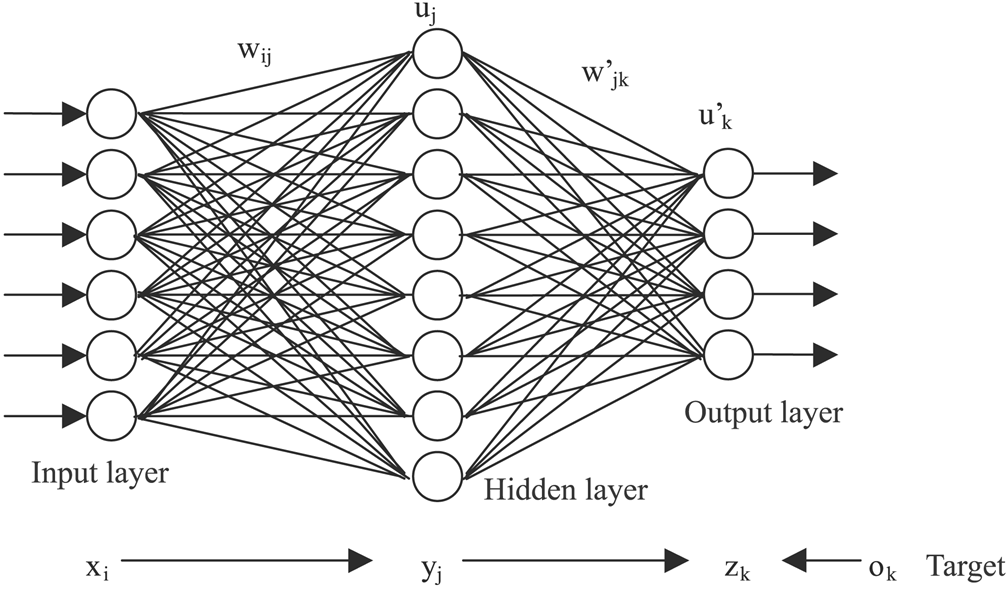
\includegraphics[width=0.5\textwidth]{neuronalesnetzwerk.png}
	\caption{Künstliches Neuronales Netzwerk\protect\cite{annpic}}
	\label{fig:Bild1}
\end{figure}

Jeder Layer besteht aus künstliche Neuronen. Diese haben ihre Namensgebung von aus der Natur stammende Neuron in Gehirnen von Lebewesen. Neuronen sind die Bausteine, aus denen die Gehirne von Lebewesen wie Fischen, Vögeln und Säugetiere zusammen gesetzt sind. Neuronen, oder auch Nervenzellen haben einen Zellkern der Zentrum der Zelle ist. Um sie herum sind Dendriten welche die Verbindung zu anderen Neuronen her stellt. Neuronen sind untereinander mit dem Axonen verbunden, welche an den enden Synapsen haben die Grenze von Axon zur Nervenzelle einen Spalt bilden. Dieser Spalt kann überwunden werden indem von der Synapse Botenstoffe abgesendet werden, die sich dann an den Rezeptor der gegenüberliegenden Synapse anhaften. Diese Übertragung findet statt wenn an der Synapse ein bestimmter Schwellenwert überschritten wurde von elektrischen Reizen, welche die Zelle abfeuert lässt. Künstliche Neuronen haben diesen Schwellenwert durch sogenannte Gewichte w\textsubscript{ij} diese sind auf den Verbindungen zwischen den Neuronen in den unterschiedlichen Layern im KNN (vgl. \ref{fig:Bild2}). Dabei steht i für die Position im Layer und j in welchen Layer sich das Neuron befindet.

\begin{figure}[htbp] 
	\centering
	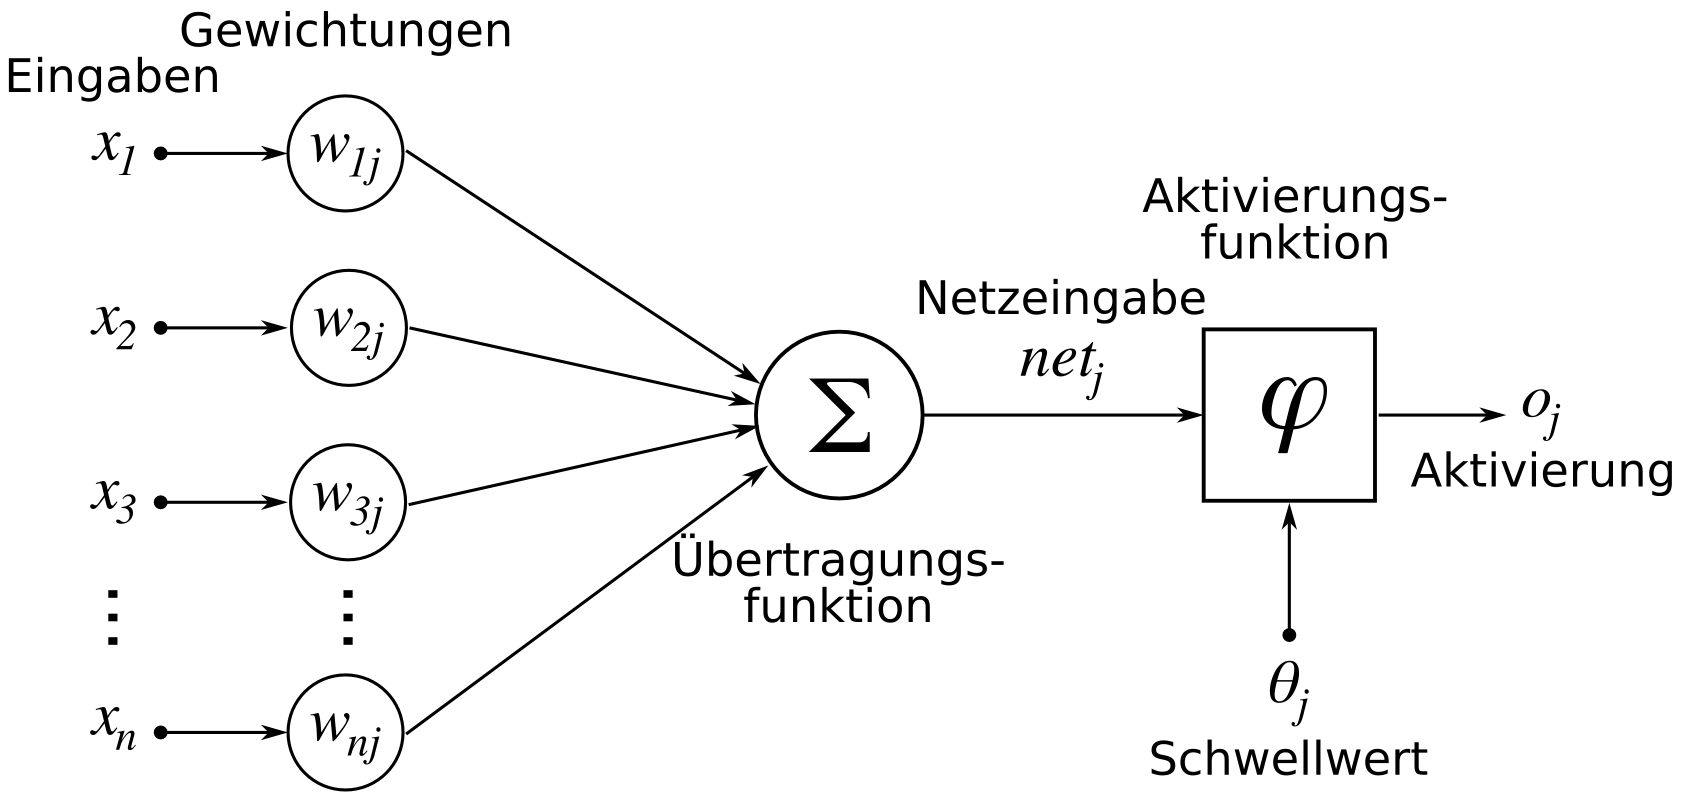
\includegraphics[width=0.5\textwidth]{Neuron.png}
	\caption{künstliches Neuron}
	\label{fig:Bild2}
\end{figure}

~\\
Jeder Layer eines KNN besteht aus mehreren Neuronen. Ein Neuron $\theta$ kann mehrere Inputs X\textsubscript{n} erhalten und produziert einen Output $\omega$\. Die Berechnungen, welche von den Neuron durchgeführt werden sind zunächst jeden Input X\textsubscript{n} mit einen Gewicht w\textsubscript{ij} zu multiplizieren. Anschließend wird die Summe von x*w gebildet. Das Ergebnis wird dann in eine Aktivierungsfunktion $\lambda$ gegeben. Ein Neuron ist definiert durch:
\\\\
\begin{math}
y\textsubscript{k} = \lambda(\sum_{j=0}^{m}(w\textsubscript{kj}+x\textsubscript{j})+b\textsubscript{k})                
\end{math}
\\\\
Die Aufgabe der Aktivierungsfunktion $\lambda$  ist es eine nicht lineare Transformation des Inputs zu erzeugen. Damit kann das KNN nicht lineare Funktionen abbilden und somit komplexere Aufgaben lösen. Es gibt unterschiedliche Aktivierungsfunktionen im folgenden werden einige aufgezählt:
\vspace{5 mm}
\begin{description}
	\item[Sigmoid-Funktion]		
	
	\begin{math}
	\sigma(x)=\frac{1}{1+exp(-x)}
	\end{math}
	\vspace{5 mm}
	\item[Softmax-Funktion]
	
	\begin{math}
	\zeta(x)\textsubscript{j} = \frac{e\textsuperscript{x\textsubscript{j}}}{\sum_{k=1}^{K}e\textsuperscript{x\textsubscript{k}}}
	\end{math}
	\vspace{5 mm}
	\item[Rectified Linear Unit (ReLU):]
	
	\begin{math}
	f(x)=\max(0,x) 
	\end{math}
	\vspace{5 mm}
	\item[Leacky Rectified Linear Unit(Leaky Relu):]
	
	\begin{math}
	f(x) = \begin{cases}
	x  	 & \quad \text{if } x > 0\\
	0.01x & \quad \text{sonst} 
	\end{cases}
	\end{math}
	\vspace{5 mm}
\end{description}
\vspace{5 mm}
Der Funktionsplot von Sigmoid Funktion kann Abb.\ref{fig:Bild3} entnommen werden. Dieser veranschaulichen den Wertebereich, welcher von den Aktivierungsfunktion angenommen werden kann und ihren Verlauf. 
\begin{figure}[htbp] 
	\centering
	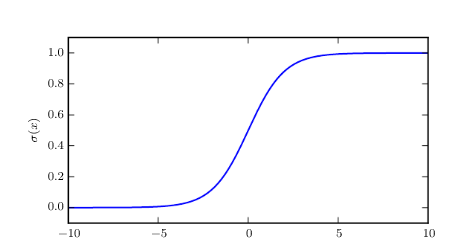
\includegraphics[width=0.8\textwidth]{sigmoid.png}
	\caption{Sigmoid Funktion}
	\label{fig:Bild3}
\end{figure}

\newpage
\subsubsection{Ziel-Funktion}\label{sec:Zielfunktion}
~\\\\
Die Ziel-Funktion oder auch Loss-Funktion genannt J($\theta$), muss differenzierbar sein wobei $\theta$ das KNN ist und J für die Zielfunktion steht. Das heißt die Funktion f: D $\to$ R ist differenzierbar an der Stelle x\textsubscript{0}. Wenn nun $f^\prime$: x $\to$ f(x) an jedem Punkt x\textsuperscript{n} ableitbar ist, ist f differenzierbar. Die Aufgabe der Ziel-Funktion ist es zu messen wie gut unsere Model $\theta$ f*(x) approximiert. Es wird der Begriff Kosten verwendet, wie viel Kosten erzeugt das Model beim Lösen der zugewiesenen Aufgabe. Die Wahl, welche Ziel-Funktion gewählt wird ergibt sich aus der Aufgabe des KNN. Diese kann beispielsweise für Klassifikations oder Regressions Aufgaben hergenommen werden. Bei Regression soll eine kontinuierliche Variable von $\theta$ als Output generiert werden, wohingegen bei Klassifikationsproblemen der Output Klassen-Labels darstellt\cite{Grundlagen}. Es gibt verschiedene Ziel Funktionen im folgenden wird die Cross Entropy Loss Function vorgestellt \cite{crossentropy}. Diese kann verwendet werden um beispielsweiße Klassikationsprobleme zu lösen. Diese ist definiert als:
\\\\
\begin{math}
\hat{q}(c\mid x)=\displaystyle\arg\min_{q(c\mid  x)}\{-\displaystyle\sum_{n}{\log q(c\textsubscript{n}\mid x\textsubscript{n})}\}
\end{math}
\\\\
Wobei  x\textsubscript{n}:n=1,...,N die Trainingsdaten sind und c\textsubscript{n}:n=1,...,N die möglichen Klassen. Der Output ist die Wahrscheinlichkeit zwischen 0 und 1, ob  x\textsubscript{i} $\in$ der bestimmten Klasse enthalten ist. Auch kann sie hergenommen um zu messen wie hoch die Differenz zwischen zwei Wahrscheinlichkeitsverteilungen ist.


\subsubsection{Backpropagation Algorithmus}\label{sec:test}
~\\\\
Um nun KNNs zu trainieren und den gewünschten Output y zu generieren wird der Backpropagation Algorithmus benutzt. Dieser zählt zu den Optimierungs Algorithmen für KNN und arbeitet schneller und effizienter auf Neuronalen Netzwerken als andere Optimierungsalgorithmen vor ihm. Das mathematische zugrundeliegende Konzept ist ein Optimierungsproblem der die partitielle Ableitung von  $\frac{\partial J}{\partial w}$, wobei J die Zielfunktion und w die Gewichte im zu optimierenden Neuronalen Netzwerk, sind. Für eine Funktion $f$(x) = y ist die Ableitung definiert als $f^\prime$(x) oder $\frac{dy}{dx}$ und gibt die Steigung der Funktion an Punkt x an. Durch die Steigung am Punkt x ist man nun in der Lage eine Änderung von der Ableitung x dahin gehend  zu optimieren \cite{Grundlagen}. Dieses Verfahren hilft dabei das KNN  dahingehen zu optimieren den gewünschten Output y zu erlangen. Dieses Ziel wird durch die Ziel-Funktion einen KNN beschrieben(vgl. \ref{sec:Zielfunktion}). Das Verfahren wird in Abb. \ref{fig:Bild4} veranschaulicht.   
\\
\begin{figure}[htbp] 
	\centering
	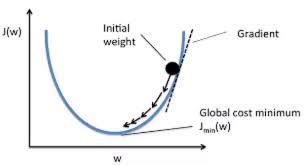
\includegraphics[width=0.5\textwidth]{gradient.png}
	\caption{Optimierung einer Zielfunktion}
	\label{fig:Bild4}
\end{figure}
\\
Wenn nun $f^\prime$(x) = 0 gibt es keinerlei Information über die Steigung. Dies ist aber kein Indiz dafür,dass $f$ ein Optimum erreicht hat. Es könnte, wie in Abbildung \ref{fig:Bild5} unten dargestellt ein lokales Minimum sein, was bedeutet, dass an diesen Punkt ein Minimum erreicht ist aber im Funktionsverlauf ein noch niedrigeres Minimum vorhanden ist. Oder einen Sattelpunkt welche einen Übergang zu einen anstieg der Funktion bildet.
Ist nun die die Funktion $f$ definiert als $f$: $\mathbb{R}$\textsuperscript{n} $\rightarrow$  $\mathbb{R}$ hat sie als Input mehrere Variablen. Die partielle Ableitung $\frac{\partial f(x)}{\partial x\textsubscript{i}}$ zeigt an wie sehr sich $f(x)$ ändert wenn x\textsubscript{i} geändert wird. Der Gradient $\nabla\textsubscript{x}f(x)$ ist ein Vektor, welcher alle partiellen Ableitungen von $f$ enthält. Nun kann f optimieren  werden, in dem, in die Richtung die Gewichte w\textsubscript{ij} von $\theta$ dahin gehen verändert werden in dem das Gradientenverfahren absteigend zu $f^\prime$(x) = 0 optimiert wird. Dieses Verfahren wird Gradient Descent genannt \cite{Grundlagen}.

\begin{figure}[htbp] 
	\centering
	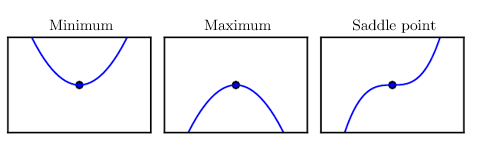
\includegraphics[width=1.0\textwidth]{saddle.png}
	\caption{Minimum,Maximum und Sattelpunkt einer Zielfunktion \protect\cite{saddleimage}}
	\label{fig:Bild5}
\end{figure}


\subsubsection{Momentum}\label{sec:momentum}
~\\\\
Momentum hat das Ziel das Gradientenverfahren des Backpropagation Algorithmus \ref{sec:test} zu beschleunigen, um ein effizienter Ergebnis herbei zu führen und ein schnelleres Lernen erreichen. Definiert ist dies durch:
\\\\
\begin{math}
v\textsubscript{t+1} =\mu v\textsubscript{t}-\epsilon\nabla$f$(\theta\textsubscript{t})
\theta\textsubscript{t+1}= \theta\textsubscript{t}+v\textsubscript{t+1}
\end{math}
\\\\
wobei $\epsilon$ $>$ 0 die Lernrate ist,  $\mu$ $\in$ [0,1] das Momentum und $\nabla$f$(\theta\textsubscript{t}$ der Gradient von $\theta\textsubscript{t}$. Je größter das Momentum, desto schneller bewegt sich der Gradient abwärts. Da dieser am Anfang einer Lernphase der üblicherweise hoch ist empfiehlt sich zunächst mit einen niedrigen Momentum zu Arbeiten da sonnst die Gefahr besteht über das globale Optimum hinaus zuschießen. Wenn nun das Training stagniert, was aus Gründe der Aufbau der Zielfunktion zurückzuführen ist das zur nähe des globalen Optimums flache Täler entstehen welche das Trainings verlangsamen und es zu keiner Verbesserung kommt, kann man durch Momentum erzwingen größere Gradienten Sprünge einzugehen. Und sich somit schneller zu einen globalen Optimum zu bewegen oder aber aus einen lokalen Optimum hinaus Richtung eines globalen Optimum zu bewegen kann Momentum benutzt werden\cite{momentum}.

\subsubsection{Regularization}
~\\\\
Ein Problem welches alle Machine Learning Anwendungen teilen ist es wenn der Trainingsalgorithmus zunächst eine gutes Trainingsergebnis erzielt, aber dann auf dem Testdatensatz ein schlechtes Ergebnis erlangt, was Overfitting genannt wird. Es gibt einige Möglichkeiten die eingesetzt werden können, welche dann aber ebenfalls auch das Trainingsergebnis verschlechtern. Man spricht davon das Model zu Regularizieren.

\begin{description}
\item[Data Argumentation]
~\\\\
Je mehr Daten beim Training verwendet werden desto mehr kann generalisiert werden. Data Argumentation heißt, dass man mehr Datensätze erstellt. Dies kann durch eine Veränderung der Trainingsdatensätze im Allgemein geschehen \cite{Grundlagen}, wenn man beispielsweise 3D-Punktwolken rotiert, um diese mehrfach zu nutzen. Eine weitere Möglichkeit ist es, bestimmte Datenpunkte in einen Datensatz ändern indem man ein Objekt, welches auf einem Bild dargestellt wird, verkleinert oder vergrößert\cite{Grundlagen}. \\
\item[Dropout]
~\\\\
Bei Dropout wird während des Lernprozess ein gewisser Prozentsatz der Neuronen in jedem Layer nicht verwendet. Dies zwingt das Netzwerk, welches sonnst die Abhängigkeiten zwischen den Neuronen lernt, eine generalisiertere Lösung zu finden\cite{dropout}.\\
\item[L2-Regularization]
~\\\\
Dabei wird das Gewicht des Neurons während des Trainings näher zu seinem Ursprung, dass heißt dem Wert seiner Initialisierung, gedrängt. Dies passiert indem ein Regularisierungswert $\Omega$ = $\frac{1}{2}||w||\frac{1}{2}$ an die Zielfunktion gehängt wird. Dieses sorgt dafür, dass während dem Training der Gewichts Vektor welche durch das Gradienten Verfahren ermittelt wird, schrumpft, was für eine höhere Varianz während des Trainings sorgt, welches wiederum das KNN dazu zwingt mehr zu generalisieren\cite{Grundlagen}.\\ 
\end{description}

\subsubsection{Batch Normalisation}
~\\\\
Wie in Kapitel \ref{sec:test} gezeigt hat das stochastischen Gradienten Verfahren Vorteile gegenüber dem normalen Gradienten Ermittlung Verfahren beim Training von KNN. Dadurch das der Input in jeden Layer abhängig von den vorherigen Layern ist können Änderungen von Werten in frühen Layern des KNN große Auswirkungen in tieferen Layern im Netzwerk haben.
Dadurch resultiert dass in Trainingsabläufen die Verteilung der Gewichte in den jeweiligen Layern verlangsamt wird. Batchnormalization soll die Werteänderung von Gewichten verringen. Dieses Problem wird auch Covariance Shift genannt. Um dies zu verhindert zeigten Sergey Ioffe und Christian Szegedy \cite{batchnorm} eine Methode, welche Batch Normalisation genannt wird. Je mehr Layer das Netzwerk hat desto stärker ist der Covariance Shift. Batch Normalisation besteht aus zwei Algorithmen. Algortithmus 1 verändert den eigentlichen Input von Layer n zu einen normalisierten Input y und Algorithmus 2 verändert das eigentliche Training eines Batch normalisierten Netzwerkes\cite{batchnorm}.
\\\\
\begin{algorithm}[H]
	Input: Werte von x über einen Mini-Batch $B$ = \{$x\textsubscript{1},...,x\textsubscript{n}$\}\\
	\begin{math}
	\mu\textsubscript{$B$}\leftarrow\frac{1}{m}\displaystyle\sum_{i=1}^{m}$x$\textsuperscript{i}
	\end{math}\\
	\begin{math}
	\sigma\textsubscript{$B$}\leftarrow\frac{1}{m}\displaystyle\sum_{i=1}^{m}($x$\textsuperscript{i} - \mu\textsubscript{$B$})\textsuperscript{2}
	\end{math}\\
	\begin{math}
	\hat{x\textsubscript{i}}\textsubscript{$B$}\leftarrow\frac{x\textsubscript{i}-\mu\textsubscript{$B$}}{\sqrt{\sigma\textsubscript{$B$} + \epsilon}}
	\end{math}\\
	\begin{math}
	$y$\textsubscript{i}\leftarrow\gamma\hat{x\textsubscript{i}} + \beta \equiv BN\textsubscript{$\gamma$;$\beta$}($x$\textsubscript{i})
	\end{math}\\
	Output: \{$y$\textsubscript{i}=BN\textsubscript{$\gamma$;$\beta$}($x$\textsubscript{i})\}
	\caption{Batch Normalisierung angewand auf x über Input bei Mini-Batch  }	
\end{algorithm}
~\\\\
In Schritt 2 des Algorithmus 1 wird der Erwartungswert für alle Inputs von Mini-Batch B berechnet und in Schritt 3 die Varianz. In Schritt 3 wird nun der der normalisierte x\textsubscript{i} berechnet welche dann mit $\beta$ und $\gamma$ multipliziert werden. Diese Werte sind neue Gewichte im Neurnonalen Netzwerk welche während des Trainingsprozesses angepasst werden. $\epsilon$ in der Gleichung in Zeile 4 ist nur dafür da damit nicht durch 0 geteilt werden kann. In Zeile 8 - 11 werden die Inferenz Schritte beschrieben, bei welchen der Minibatch des Trainings ersetzt wird \cite{batchnorm}. In Abb. \ref{fig:Bild6} ist veranschauchlicht wie die Batch-Normalization-Layer in das KNN eingebaut werden. 

\begin{figure}[htbp] 
	\centering
	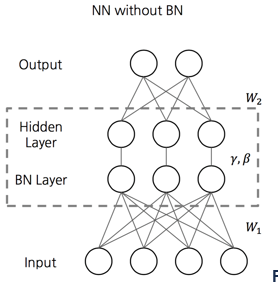
\includegraphics[width=0.3\textwidth]{batchnorm.png}
	\caption{Neuronales Netzwerk mit Batch-Normalization-Layer\protect\cite{batchnormweb}}
	\label{fig:Bild6}
\end{figure}

\subsection{Datenformat Punktwolken}\label{sec:punktwolken}

Punktwolken sind eine Menge von N Punkten, welche im Vektorraum dargestellt werden können. Jeder Punkt n $\in$ N wird durch seine (x,y,z) Koordinaten im Euklidischen Raum dargestellt. Punkte können zusätzliche Features gegeben werden, wie Farbe oder Material. Es gibt unterschiedliche Dateiformate, welche für die Abspeicherung von Punktwolken herangezogen werden können bespiele dafür sind PLY, STL oder OBJ. Das Polygon File Format(PLY) speichert die einzelnen Koordinaten in einer Liste, welche Vertex List genannt in. In Abb. \ref{fig:Bild7} kann eine Beispieldatei entnommen werden in der dieser Aufbau dargestellt ist. 
\\
\begin{figure}[htbp] 
	\centering
	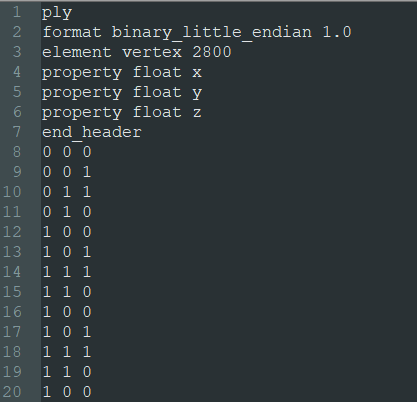
\includegraphics[width=0.3\textwidth]{plyexample.png}
	\caption{Polygon File Format}
	\label{fig:Bild7}
\end{figure}
\\
Punktwolken können als Menge betrachtet werden. Die jeweiligen Punkte sind geordnet in dieser Listen gespeichert jedoch spielt es keine Rolle für den Punktwolkencompiler bei der Visualisierung der Liste an welcher Listenposition ein jeweiliger Punkt geführt wird, die Liste wird jedes mal gleich angezeigt, egal welche Permutation der einzelnen Punkte in der Liste durchgeführt wird. In Abb. \ref{fig:Bild8} kann eine visualisierte Punktwolke eines Tabakblattes entnommen werden. 
\\
\begin{figure}[htbp] 
	\centering
	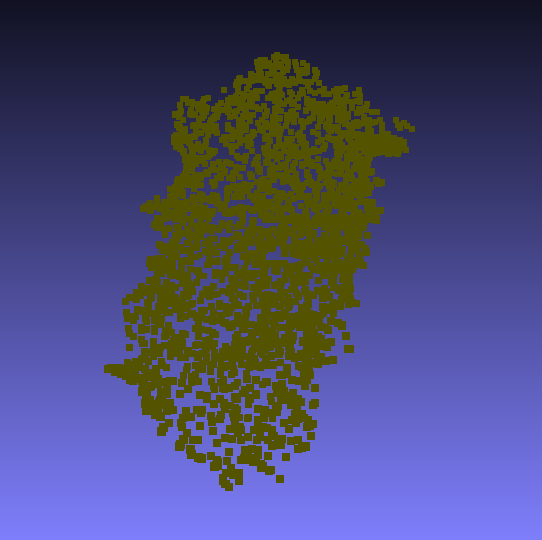
\includegraphics[width=0.3\textwidth]{leaf1.png}
	\caption{Punktwolke eines Tabakblattes}
	\label{fig:Bild8}
\end{figure}
\newpage
\subsubsection{Datenaufnahme von Tabakpflanzen}
~\\\\
Die Punktwolken können Beispielsweise von den TERRA-REF Feld Scanner von der University von Arizona Maricopa Agricultural Center and USD Arid Land Researh Station in Maricopa aufgenommen werden. In Abb. \ref{fig:Bild9} ist  Recht eine Skizze dargestellt. In Abb. \ref{fig:Bild9} Links ist der Scankopf des TERRA-REF dar gestellt. 
 

\begin{figure}[htbp] 
	\centering
	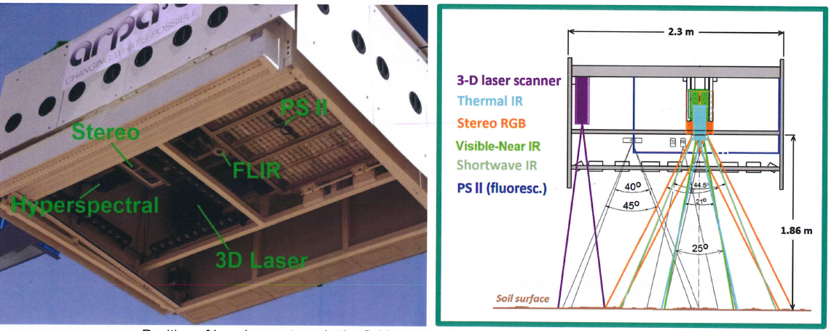
\includegraphics[width=0.5\textwidth]{lematech_2.png}
	\caption{Scankopf und Scanaufbau für die 3D-Punktwolken Gewinnung}
	\label{fig:Bild9}
\end{figure}

Der 3D Laser Scanner erzeugt 3D Punktwolken. Dabei werden die Objekte durch den Scanner erfasst und eine 3D Repräsentation, welche durch Punkte in einen 3 Dimensionalen Koordinaten System erfasst werden können, dargestellt. Dabei wird ein Laser über das zu scannende Objekt gefahren durch reflektion des Laserstrahls auf der Oberfläche des Objektes können x,y,z Koordinaten des jeweiligen Punktes auf den Objekt bestimmt werden. Da nun beim Scannen eines Objektes durch andere Objekte die Oberfläche verdeckt sein können. Wie beispielsweise beim Scannen von Tabakpflanzen, Blätter den Scankopf es nicht Möglich macht Objekte unterhalb dieses zu erreichen. Können Scans unvollständig sein. Dieses Problem für zu den Ziel dieser Arbeit, eine Möglichkeit zu Prüfen diese unvollständigen Punktwolken zu vervollständigen. Genaueres zum diesen Thema in Kapitel \ref{sec:rekdaten}. 

\newpage
\subsubsection{Die Schwierigkeit bei mit 3D-Data bei Machine Learning Ansätzen}\label{sec:3dprobleme}
~\\\\
Vergleicht man 3D-Data auf ihre Dimensionalität mit anderen Datenformaten wie Bild,- Audio-, und Textdateien steigt der Informationsgehalt und dadurch auch die Komplexität für das Anwenden von Maschine Learning Algorithmen enorm. Besonders bei Nicht-Euklidischen 3D-Daten wie Punktwolken, welchen keine Struktur zu Grunde liegt ist dieses gegeben \cite{3dprob}.
\\\\
Wie im Kapitel \ref{sec:punktwolken} gezeigt, sind Punktwolken als Menge gespeichert, in der keine Relation untereinander besteht. Was bedeutet, dass es für den Punktwolkencompiler nicht von Relevanz ist auf welchem Platz die einzelnen Punkte abgespeichert werden. Die Punktwolke wird immer gleich angezeigt, egal in welcher Permutation der einzelnen Punkte abgespeichert abgespeichert werden. Vergleicht man nun ein Bild mit 512 Pixeln und 3 RGB-Farbkanälen ist einer Dimension von 391680 erreicht. Vergleicht man dies mit einer Punktwolke in einen 125 cm \textsuperscript{3}großen Bereich. Da die einzelen Koordianten eines Punktes als Rationale Zahlen dargestellt werden und rationale Zahlen abzählbar unendlich sind ist der Suchraum unendlich groß. Dies führt zu einen erheblichen mehr Aufwand für Machine Learning Ansätzen wie, Deep Learning für Punktwolken.
\\\\
Ein weitere Schwierigkeit, die für Deep Learning mit Punktwolken besteht ist, dass die aus Kapitel Convolutional Neural Network beschrieben Convolutionel-Layer einen großen Beitrag bei dem Fortschritt von Deep Learning gebracht hat. Da sie helfen die Strukturen von strukturierten Daten zu lernen und den latenten Raum zu entdecken. Da jedoch Pointclouds unstrukturiert sind hilft es nicht unbedingt diese Tools auch bei Punktwolken einzusetzen\cite{3dgan}.  

\subsection{Convolution Neural Networks}

Convolution Neural Netzworks(CNN) sind eine besondere Art von künstlichen neuronalen Netzwerken, sie sind dafür konzipiert auf Datensätzen zu arbeiten welche in eine Matrix Form gebracht worden sind. Der Input eines CNN können beispielsweise Bilder sein welche durch die Matrix A =
$
\begin{bmatrix}
a_1	& a_1	& \dots	 & a_n     \\
b_1	& b_2 	& \dots  & b_n	  \\
\vdots	& n_n 	& \ddots & \vdots \\
x_1 	& x_2 & x_3	 & x_n
\end{bmatrix}
$
\\\\dargestellt werden. Jedes Element x\textsubscript{ij} stellt einen Pixel eines Bildes da, wobei x\textsubscript{n} $\in$ [0,255] . Die Matrix A\textsuperscript{w$\cdot$b$\cdot$c} stellt w$\cdot$b$\cdot$c = N dimensionale Matrix da. Wobei w die Länge und b Breite des Bildes entspricht. c sind die Farbspektren eines Bildes und sind in einen RGB-Farbraum 3 beziehungsweiße in einen schwarz-weiß Bild 1. Nachdem  der Input eines CNN definiert ist kommt nun der Aufbau. CNN setzen sich aus mehrere Schichten von Convolution Layern zusammen. Ein Netzwerk kann mehrere N-Layer haben. Wobei jeder Layer aus mehreren Convolution oder auch Kernels genannt, zusammengesetzt ist. Ein Aufbau kann aus Abbildung \ref{fig:Bild10} entnommen werden\cite{Grundlagen}.

\begin{figure}[htbp] 
	\centering
	\includegraphics[width=1.0\textwidth]{convol.png}
	\caption{Convolutional Neural Network}
	\label{fig:Bild10}
\end{figure}

Die Kernels, also die einzelnen Filter, von denen jeder der N-Layer k besitzt sind K\textsuperscript{n$\cdot$n} Matrizen jedes k\textsubscript{ij} in einem Filter einspricht einen, aus den üblichen Neuronalen Netzwerk Architektur bekannten Gewichte. Diese Gewichte werden dann durch den Backprobagation-Algorithmus in der Trainingsphase des Netzwerkes angepasst um den Verlust der Loss-Funktion durch bestimmten des Gradianten zu minimieren. Das durch die Abbildung \ref{fig:Bild2} dargestellte Subsampling ist der Output aus den Convolutional Layern\cite{Grundlagen}. 
\\\\
Da Input und Kernel unterschiedliche Größen haben und man den gesamten Input mit den Kernel abdecken möchte, bewegt sich der Filter um s Position auf den Input und führt erneut einen Berechnungschritt durch. Dieser Vorgang wird Stride genannt. An jeder Position wird das Produkt von jeden x\textsubscript{ij} des Input und k\textsubscript{ij} des Kernel durchgeführt.  Anschließend werden alle Produkte aufsummiert. In Abbildung \ref{fig:Bild11} ist dieser Vorgang verdeutlicht. Zusätzlich gibt es die Möglichkeit für das sogenannte Zero Padding P. Dabei werden mehrere 0 um die Input Feature Map, am Anfang und Ende der Axen anfügt. Dies ist notwendig wenn Kernel und Input Größe nicht kompatible zueinander sind. Die Anzahl der möglichen Positionen ergeben sich aus Kernel Größe und den Input des jeweiligen Kernel sowie des Strides. Die Output Größ W kann berechnet werden durch W = (W-F+2P)/s+1. Wobei F für die Größe des Kernel steht \cite{conv}.

\begin{figure}
	\centering
	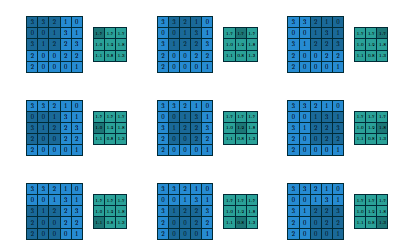
\includegraphics[width=0.8\textwidth]{conv.png}
	\caption{Convolution Beispiel\protect\cite{conv}}
	\label{fig:Bild11}
\end{figure}
~\\\\
Um  besser zu verstehen welche Auswirkungen die Anzahl der Kernels in Layer n auf die Größe des Outputs von n und die Anzahl der Kernels in Layer n+1 für den nächsten Layer haben, wird ein Beispiel aufgezeigt. Der erste Layer hat 20 Kernels mit der Größe 7x7 und Stride 1. Der Input A für einen Kernel K ist ein 28x28 Matrix. Der Output aus diesen Filter sind 20 22X22 Feature Maps. Würde der Input ein 28x28x3 Bild mit 3 RGB Channels sein, der Output 60 22x22 Feature Maps. Allgemein kann Convolution Layer als Supsampling gesehen werden und Stride gibt an wieviele Dimensionen bei diesen Prozess pro Convolution Layer entfernt werden soll. Der letzte Layer ist ein fully-connected Layer welcher den typischen Anforderungen von ANN entspricht \cite{conv}.  
\\\\
Transposed Convolution, auch genannt Fractionally Strided Convolution oder Deconvolution ist eine Umkehrfunktion von der üblichen Convolution. Es verwendet die gleichen Variablen wie Convolution. Dabei wird ein Kernel K mit der Größe N x N definiert der Input I mit der Größe N x N und Stride s = 1. Deconvolution kann wie Convolution angesehen werden mit  Zero Padding auf dem Input.  Das in Abbildung \ref{fig:Bild12} gezeigte Beispiel zeigt einen deconvolution Vorgang mit eine 3x3 Kernel über einen 4x4 Input. Dies ist gleich mit einen Convolution Schritt mit einen 3x3 kernel auf einen 2x2 Input und einer 2x2 Zero Padding Grenze. Convolution ist Supsampling und mit Deconvolution wird Upsampling betrieben. Durch diesen Schritt kommt es zu einer Dimensionserhöhung des Inputs. Die Gewichte der Kernels bestimmen wie der Input transfomiert wird. Durch mehrere Schichten von Deconvolution Layer kann von einer Input Größe NxN auf eine Output Größe KxK, wobei K $>$ N mit Abhängigkeit von Kernel und Stride abgebildet werden\cite{conv}. 

\begin{figure}[htbp] 
	\centering
	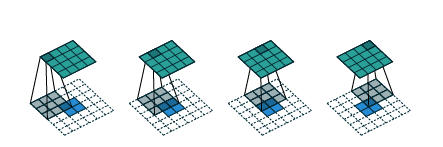
\includegraphics[width=1.0\textwidth]{decon.png}
	\caption{Deconvolution Beispiel \protect\cite{conv}}
	\label{fig:Bild12}
\end{figure}
\newpage

\subsection{Autoencoder}\label{sec:autoencoder}

Autoencoder gehören zu den generativen Modellen im Bereich des Machine Learnings. Generative Modelle haben das Ziel eine Wahrscheinlichkeitsverteilungen zu erlernen. Anschließend kann diese als ein Modell genutzt werden um Samples aus dieser zu erzeugen. Die Modelle können dabei beispielsweise auf ANN oder Markov Chains trainiert werden\cite{Grundlagen}. Im folgenden liegt der Fokus auf ANNs. Allgemein gehalten können jegliche Typen von Daten wie Text, Bild oder Audiodateien für generative Modelle herangezogen werden. Es gibt unterschiedliche Typen von generativen Modellen, welche sich vom Aufbau des Neuronalen Netzwerk und der Zielfunktion unterscheiden. Beispiele dafür sind Boltzmann Maschine, Autoencoder oder Deep Belief Networks\cite{Grundlagen}. 
\\\\
Autoencoder sind eine andere Art von Model aus den Bereich der generativen Modelle. Ihre Aufgabe besteht darin einen Input zu komprimieren und aus der komprimierten Information den Input wieder herzustellen. Die Technik auf welche Autoencoder zurückgreifen, nennt sich Dimensionreduktion. Dabei wird die Dimension der Daten so reduziert um Informationen bei zu behalten, welche als relevant gelten. Diese Technik findet auch in anderen Machine Learning Anwendung, wie beispielsweise der Principale component anaysis(PCA) Anwendung\cite{dimreduction}.  Ein Autoencoder besteht aus 2 Bestandteilen. Erstens einen Encoder e parametrisiert mit $\phi$ welcher einen Input x $\in$ von $x\textsuperscript{i}$ wo x ein Vektor der Länge i ist und damit die Input Dimension bestimmt. Dieser wird durch den Encoder auf einen Vektor $z\textsuperscript{k}$ abgebildet wobei k<i ist. Zweitens der Decoder d parametrisiert durch  $\theta$, bekommt als Input $z\textsuperscript{k}$ und bildet z auf $x\textsuperscript{l}$ ab wobei l = i. Und somit die gleiche Dimension wie der Input. Aufgabe ist es nun, dass der Encoder den Input z so gut komprimiert, dass der Encoder es schafft das x $\thickapprox$ z. Eine grafische Darstellung kann aus Abb. $\ref{fig:Bild13}$ entnommen werden\cite{Grundlagen}. 
\\\\
Die Parameter $\phi$ und $\theta$ werden durch den in Kapitel \ref{sec:test} vorgestellten Algorithmus trainiert und erlernt so können beispielsweise durch Fully-Connected-Layer, Convolutional-Layer oder Deconvolutional-Layer modelliert werden. Eine Metrik um zu messen wie das Model seine Aufgabe erfüllt, könnte beispielsweiße die Cross-Entropy-Funktionen sein welche schon in Kapitel \ref{sec:Zielfunktion} vorgestellt worden ist. Weitere spezifische Zielfunktionen für Autoencoder welche mit 3D Punktwolken arbeiten und für die folgende Arbeit von belangen sind, werden nun vorgestellt.

\begin{figure}[htbp] 
	\centering
	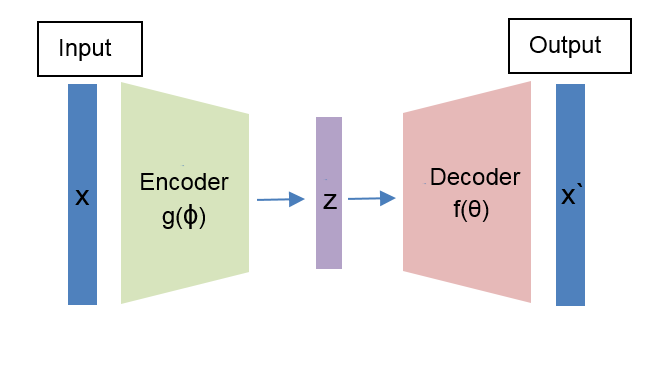
\includegraphics[width=1.0\textwidth]{autoencoder.png}
	\caption{Autoencoder}
	\label{fig:Bild13}
\end{figure}
~\\\\
Bei Punktwolken als Datentyp erzielt die Cross-Entropy-Funktion keine guten Ergebnisse da diese invariant zu ihrer Permutation sind. Da dieser Arbeit der Input 3d Pointcloud sind und diese Sets  invariant zu ihren Permutationen sind. Ändert sich Anordnung meiner einzelnen Punkte in mein Set bleibt das dargestellte Ergebnis unverändert.  Deshalb kann nicht auf übliche Zielfunktionen welche für strukturierte Daten wie Bilder verwendet werden, zurück gegriffen. Die Herausforderung besteht darin zwischen zwei unterschiedliche Sets von Punkten heraus zu finden, wie hoch die Diskrepanz zwischen den beiden Sets ist\cite{invariant}. 
\\\\
Eine Möglichkeit, speziell für Autoencoder, welche mit Punktwolken arbeiten, ist die Earth Mover Distance(EMD). Bei dieser sind X\textsubscript{1} und X\textsubscript{2} zwei Punktwolken mit jeweils x\textsubscript{n} definierten Punkten\cite{autoencoderloss}. Definiert ist sie durch die Funktion:
\\\\
\begin{math}
d\textsubscript{EMD}=\min_{\theta : X\textsubscript{1}\rightarrow X\textsubscript{2}}  \sum_{x\in X\textsubscript{1}}|| x - \theta(x)||\textsubscript{2};wobei\;\theta: X\textsubscript{1} \rightarrow X\textsubscript{2}\, bijektiv\, ist 
\end{math}
\\\\
Grafisch kann man sich die Berechnung wie in Abb. \ref{fig:Bild14} darstellen. Ein Punkt von x\textsubscript{n} $\in$ X\textsubscript{1} wird den nähsten Punkt y\textsubscript{n} $\in$  X\textsubscript{2} zugewiesen. Wobei die Distanz durch die Euklidische Distanz der jeweiligen Punkte ermittelt wird.
 
\begin{figure}[htbp] 
	\centering
	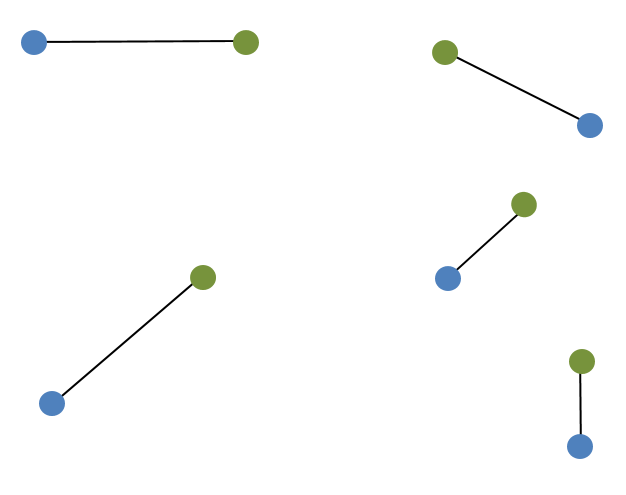
\includegraphics[width=0.5\textwidth]{emd_distance.png}
	\caption{Earth Mover Distance}
	\label{fig:Bild14}
\end{figure}
		
Eine weitere Möglichkeit ist die Chamfer Distance(CD). Wie auch zuvor sind  X\textsubscript{1} und X\textsubscript{2} zwei Punktwolken mit jeweils x\textsubscript{n} definierten Punkten\cite{autoencoderloss}. Definiert ist sie durch die Funktion:
\\\\
\begin{math}
d\textsubscript{CD}(X\textsubscript{1},X\textsubscript{2})=\sum_{x\in X\textsubscript{1}} \min_{y \in X\textsubscript{2}}||x-y|| + \sum_{y\in X\textsubscript{2}} \min_{x \in X\textsubscript{2}}||x-y||
\end{math}
\\\\
Der Unterschied ergibt sich zwischen den beiden Metriken, dass bei der EMD von der Ausgangswolke die Punkte zu der anderen jeweils optimiert werden. Wohingegen bei der CD die Distanzen von und zu der Ausgangspunktwolke berechnet werden. Dies geht aus den Abb. \ref{fig:Bild15} hinaus in welche die Distanzberechnung der einzelnen Punkte dargestellt wird\cite{autoencoderloss}.

\begin{figure}[htbp] 
	\centering
	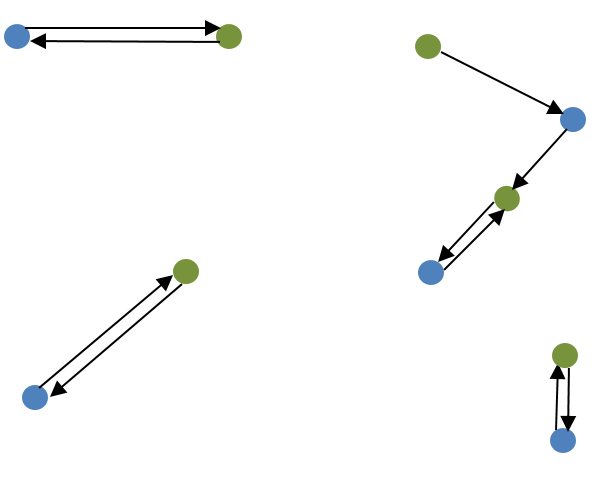
\includegraphics[width=0.5\textwidth]{champfer.png}
	\caption{Chamfer Distance}
	\label{fig:Bild15}
\end{figure} 
\newpage
\subsection{Generative Adversarial Network}
In den letzten Jahren konnte sich das GAN als best practice Ansatz bei den generativen Modellen herausarbeiten was Performancegründe bei der Trainierbarkeit und Qualität der generierbaren Daten zu Grunde liegt\cite{Grundlagen}. Die Modelle arbeiten nach der Maximum Likelihood Schätzverfahren(ML-Schätzer) in dem die Parameter $\theta$ dahingegen angepasst werden, dass die unsere beobachtetet Daten am ehesten passen. Man kann ML-Schätzer als Kulback-Leibler(KL) Divergenz darstellen und das generative Modelle das Ziel haben die KL Divergenz zwischen den Trainingsdaten P\textsubscript{r} und den generierten Daten P\textsubscript{g} zu minimieren.Diese ist definiert durch:
\\\\
\begin{math}
KL(P\textsubscript{r}||P\textsubscript{g})=\int_x P\textsubscript{r}log\frac{P\textsubscript{r}}{P\textsubscript{g}}dx                     
\end{math}
\\\\
Ein GAN besteht besteht aus zwei KNN, dem Discriminator D und dem Generator G. Das Ziel des G ist es, Daten x zu erzeugen, welche nicht von Trainingsdaten y unterschieden werden können. Dabei wird eine vorangegangene Input Noise Variable p\textsubscript{z}(z) verwendet, welche eine Abbildung zum Datenraum G(z;$\Phi$\textsubscript{g}) herstellt. Dabei sind $\Phi$\textsubscript{g} die Gewichte des neuronalen Netzwerkes von G. Der Discriminator hat die Aufgabe zu unterscheiden, ob der jeweilige Datensatz von G erzeugt wurde und somit ein fake Datensatz ist, oder von Trainingsdaten y stammt\cite{goodfellow2014}. Die Zusammensetzung zwischen den beiden Netzwerken kann aus Abbildung \ref{fig:Bild20} entnommen werden.
\\
\begin{figure}[htbp] 
	\centering
	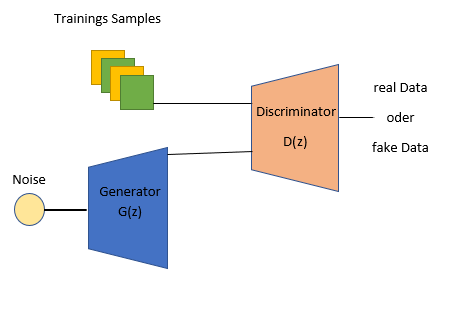
\includegraphics[width=0.5\textwidth]{GAN_GRUNDAUFBAU.png}
	\caption{Generativ Adverserial Network}
	\label{fig:Bild20}
\end{figure}
\\
Der Discriminator ist definiert durch D(x;$\Phi$\textsubscript{d}). Wobei $\Phi$\textsubscript{d} die Gewichte des Descriminators sind und D(x) die Wahrscheinlichkeit ist, dass x von den Trainingsdaten stammt und nicht von p\textsubscript{g}. Die Wahrscheinlichkeitsverteilung für unsere Trainingsdaten ist p\textsubscript{r}.  Im Training werden dann $\Phi$\textsubscript{d} so angepasst, dass die Wahrscheinlichkeit Trainingsbeispiele richtig zu klassifizieren maximiert wird. Und $\Phi$\textsubscript{g} wird dahingehen trainiert die Wahrscheinlichkeit zu minimieren, so dass D erkennt dass Trainingsdatensatz x von G erzeugt wurde. Mathematisch ausgedrückt durch log(1 - D(G(z))). Die gesamte Loss-Funktion des vanilla GAN ist definiert als
\\\\
\begin{math}
min\textsubscript{G} max\textsubscript{D}V(D,G)=E\textsubscript{x$\sim$p\textsubscript{data}(x)}[logD(x)]  + E\textsubscript{z$\sim$p\textsubscript{z}(z)}[log(1-D(G(z))]
\\\\             
\end{math}
diese beschreibt ein Minmax Spiel zwischen G und D. Welches das globale Optimum erreicht hat wenn p\textsubscript{g} = p\textsubscript{r}. Das heißt, wenn die Datenverteilung, welche von G erzeugt wird, gleich der unserer Trainingsdaten ist\cite{goodfellow2014}. Das Training erfolgt durch den folgenden Algorithmus:
\\
\begin{algorithm}[H]
	\For{Anzahl von Training Iterationen}{\For{k Schritte}{$\bullet$Sample minibatch von m noise  Samples z\textsuperscript{(1)},...,z\textsuperscript{(m)}von noise p\textsubscript{g}(z)\\
	$\bullet$ Sample minibatch von m Beispielen x\textsuperscript{(1)},...,x\textsuperscript{(m)}von Daten Generationsverteilung p\textsubscript{data}(x)\\
    $\bullet$ Update den Discriminator zum aufsteigenden stochastischen Gradianten:\\
\begin{math}
\nabla\textsubscript{$\Phi$\textsubscript{d}}\frac{1}{m}\sum_{i=1}^{m}[logD(x\textsuperscript{(i)})+log(1-D(G(z\textsuperscript{(i)})))]
 \end{math}

}$\bullet$ Sample minibatch von m noise Samples z\textsuperscript{(1)},...,z\textsuperscript{(m)} von noise p\textsubscript{g}(z)\\$\bullet$ Update den Generator mit den absteigenden stochastischen Gradianten: \\\begin{math} 
\nabla\textsubscript{$\Phi$\textsubscript{g}}\frac{1}{m}\sum_{i=1}^{m}log(1-D(G(z\textsuperscript{(i)})))\end{math}}
		\caption{Minibatch stochastic gradient descent Training für Generative Adversarial Networks. Die Anzahl der Schritte welche auf den Discriminator angewendet wird ist k }	
\end{algorithm}

Beim Training wird ein stochastischer Minibatch von mehren Trainingsdaten gleichzeitig erstellt. Dies soll dabei helfen, dass der Generator sich nicht auf bestimmte Gewichte fest fährt und auf Trainingssätze kollabiert. So weisen die erzeugten Daten mehr Variationen auf \cite{improvingan}. D wird zunächst in einer inneren Schleife auf n Trainingsätzen trainiert, womit man Overfitting von D vermeiden will, was zur Folge hätte, dass D nur den Trainingsdatensatz kopieren würde. Deshalb wird k mal D optimiert und ein mal G in der äußeren Schleife. 
\\\\
Ein möglicher Aufbau von GAN wird in Abbildung \ref{fig:Bild21} dargestellt. Dies ist das sogenannte Deep Convolution GAN(DC GAN), welches dafür konzipiert wurde auf Bilddaten zu arbeiten. Dabei besteht der Generator aus mehren Schichten von Deconvolution Layern. Welche den Input Noise Variable p\textsubscript{z}(z) auf y abbildet. D besteht aus mehren Schichten von Convolution Layern und bekommt als Input die Trainingsdaten, oder die von G erzeugten Y, und entscheidet über die Klassifikation\cite{dcgan}.

\begin{figure}[htbp] 
	\centering
	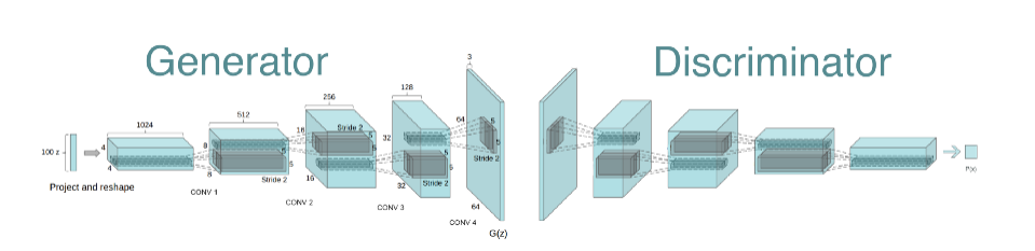
\includegraphics[width=1.0\textwidth]{dcgan1.png}
	\caption{Deep Convolutional GAN}
	\label{fig:Bild21}
\end{figure}

Wie unter Generativen Modellen gezeigt wurde kann das asymmetrische Verhalten der KV Divergenz zu schlechten Trainingsergebnissen führen. Goodfellow \cite{goodfellow2014} zeigte, dass sich die MinMax Loss-Funktion des GAN auch als Jensen-Shannon Divergenz(JS Divergenz) darstellen lässt. Diese ist definiert als
\\\\
\begin{math} D\textsubscript{JS}(P\textsubscript{r}|| P\textsubscript{g}])=\frac{1}{2}D\textsubscript{KL}(P\textsubscript{r}|| \frac{P\textsubscript{g}+P\textsubscript{r}}{2}])+D\textsubscript{KL}(P\textsubscript{q}|| \frac{P\textsubscript{g}+P\textsubscript{r}}{2}])  
\end{math}
\\\\
wobei P\textsubscript{r} die Wahrscheinlichkeitsverteilung der Trainingsdaten ist und P\textsubscript{g} die des Generators. Huzár \cite{sha} zeigte, dass durch das symmetrische Verhalten der JS Divergenz ein potentiell besseres Trainingsergebnis entstehen kann, im Vergleich zu der KL Divergenz. Damit zeigte er weshalb GANs im Vorteil gegenüber anderen generativen Modellen sind. Abbildung \ref{fig:Bild21} veranschaulicht dieses Konzept. Der linke Graph zeigt 2 Normal Verteilungen. In der Mitte wird die KV Divergenz der beiden Normal Verteilungen dargestellt.  Rechts ist die JS Divergenz der Beiden dargestellt. Man sieht sehr gut das asymmetrische Verhalten der KV und das symmetrische der JS. Dadurch lassen sich aussagekräftigere Gradianten bestimmen, welche zum Optimieren von D und G benötigt werden\cite{sha}. 
 
\begin{figure}
	\centering
	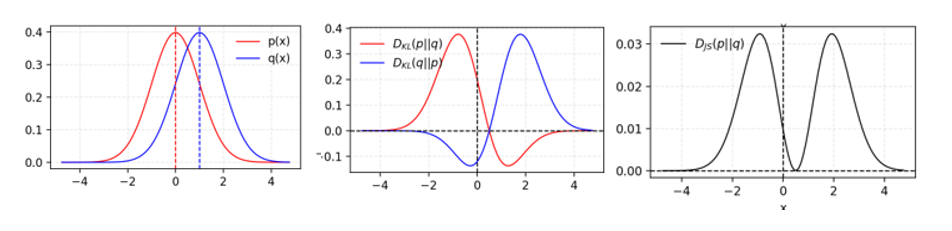
\includegraphics[width=1.0\linewidth]{KLdiv}
	\caption{KL Divergenz und JS Divergenz}
	\label{fig:Bild21}
\end{figure}

\subsubsection{Probleme mit Generative Adverserial Networks}\label{sec:problemegan}
~\\\\
Wie auch anderen generativen Modelle haben auch GANs noch Schwächen bezüglich der Trainingsabläufe und der Qualität der generierten Daten. Im Folgenden wird auf einige Probleme eingegangen welche im darauffolgenden Kapitel Lösungsansätze aufgezeigt werden. 
\\
\begin{description}	

\item[Equilibrium]
~\\
D und G betreiben ein MinMax Spiel. Beide versuchen das Nash Equilibrium zu finden. Dies ist der bestmögliche Endpunkt in einen nicht kooperativen Spiel. Wie in dem Fall von GAN wäre das wenn  p\textsubscript{g} = p\textsubscript{r}. Es wurde gezeigt, dass das Erreichen dieses Punktes sehr schwierig ist, da durch die Updates der Gewichte mit den Gradianten der Loss-Funktion starke Schwingungen der Funktion enstehen können. Dies kann zur Instabilität für das laufende Training führen \cite{improvingan}.   
\\
\item[Vanishing gradient]
~\\
Dies beschreibt das Problem, wenn D perfekt trainiert ist mit  D(x) = 1, $\forall \in p\textsubscript{r}$ und D(x)=0 $\forall x \in p \textsubscript{g}$. Die Loss-Funktion würde in diesem Fall auf 0 fallen und es gäbe keinen Gradianten, für den die Gewichte von G angepasst werden können. Dies verlangsamt den Trainingsprozess bis hin zu einem kompletten Stopp des Trainings. Würde D zu schlechten trainiert mit  D(x) = 0, $\forall \in p\textsubscript{r}$ und D(x)=1 $\forall x \in p \textsubscript{g}$. Bekommt G kein Feedback über seine Leistung bei der Datengeneration hat er keine Möglichkeit p\textsubscript{r} zu erlernen \cite{improvingan}.
\\
\item[Mode Collapse]
~\\
Während des Trainings von GAN kann es dazu kommen, dass der Generator möglicherweise auf eine Einstellung seiner Gewichte fixiert wird und es zu einem sogenannten Mode Collapse führt. Was zur Folge hat, dass der Generator sehr ähnliche Samples produziert \cite{wasserstein}.
\\
\item[Keine aussagegräftigen Evaluations Metriken]
~\\
Die Loss Funktion der GANs liefert keine aussagekräftigen Evaluationsmöglichkeit über den Fortschritt des Trainings. Bei  discriminativen Modellen im üblichen Maschine Learning besteht die Möglichkeit Validierungsdatensätze zu verwenden und an diesen die Genauigkeit des Modells zu testen. Diese Möglichkeit besteht bei GANs nicht\cite{metrics}.
\end{description}

\subsubsection{Lösungsansätze für Generative Adverserial Networks Probleme}
~\\\\
Nun werden einige Techniken aufgezeigt, welche die unter Abschnitt Probleme mit GAN genannten Schwierigkeiten angehen und zu einem effizienteren Training führen, damit eine schnellere Konvergenz während des Trainings erreicht wird.
\\
\begin{description}
\item[Feature matching]
~\\
Dies soll die Instabilität von GANS verbessern und gegen das Problem des Vanishing Gradient angehen. G bekommt eine neue Loss-Funktion und ersetzt die des üblichen Vanilla GAN. Diese soll G davon abhalten, sich an D über zu trainieren und sich zu sehr darauf zu fokussieren, D zu täuschen und gleichzeitig auch versuchen die Datenverteilung der Trainingsdaten abzudecken\cite{improvingan}.\\

\item[Minibatch discrimination] 
~\\
Um das Problem des Mode Collapse zu umgehen, so dass es nicht zu einem Festfahren der Gewichten von G kommt, wird beim Trainieren die Nähe von den Trainingsdatenpunkten gemessen. Anschließend wird die Summe über der Differenz aller Trainingspunkte genommen und dem Discriminator als zusätzlicher Input beim Training hinzugegeben \cite{improvingan}.\\

\item[Historical Averaging]
~\\
Beim Training werden die Gewichte von G und D aufgezeichnet und je Trainingsschritt i verglichen. Anschließend wird an die Lossfunktion je Trainingschritt die Veränderung zu i-1 an die Loss-Funktion addiert. Damit wird eine zu starke Veränderung bei den jeweiligen Trainingsschritten bestraft und soll gegen ein Model Collapse helfen \cite{improvingan}.\\

\item[One-sided Label Smoothing]
~\\
Die üblichen Label für den Trainingsdurchlauf von 1 und 0 werden durch die Werte 0.9 und 0.1 ersetzt. Dies führt zu besseren Trainingsergebnissen. Es gibt derzeit nur empirische Belege für den Erfolg, jedoch nicht weshalb diese Technik besser funktioniert\cite{improvingan}.\\

\item[Adding Noises]
~\\
Noise an den Input von D zu hängen kann gegen das Problem des Vanishing gradienten helfen und das Training verbessern\cite{improvingan}.\\

\item[Wasserstein-GAN]
~\\
Die Wasserstein Metric oder auch Earth Mover Distance(EMD) genannt misst die Minimum Kosten welche entstehen wenn man Daten von der Datenverteilungp p\textsubscript{r} zur Datenverteilung p\textsubscript{g} überträgt. Es wird oft auch von Masse oder Fläche gesprochen, welche von p\textsubscript{r} zu p\textsubscript{g} getragen wird. Definiert ist sie durch:
\\\\
\begin{math} 
$
W(p\textsubscript{r},p\textsubscript{g})=$\inf_{\gamma\sim\prod(P\textsubscript{r},P\textsubscript{g})}$E\textsubscript{(x,y)$\sim\gamma$}[$\parallel$x - y$\parallel$]
$
\end{math}
\\\\
p\textsubscript{r} steht für die reale Datenverteilung zu welche uns Daten im Form von Trainingsdaten zur Verfügung stehen und p\textsubscript{g} steht für die generierte Datenverteilung welche von einen Model erzeugt wird. Dabei wird nun das Infinum von allen möglichen Transportplänen $\gamma$ welche in $\prod$ enthalten sind ausgewählt, welche der kostenkünstige Plan ist die Daten von p\textsubscript{g} zu p\textsubscript{r} zu übertragen. Vorteile sind unter anderem, dass der Gradient gleichmäßiger ist und das WGAN lernt besser auch wenn der Generator schlechtere Daten erzeugt im Vergleich zum üblichen GAN\cite{wasserstein}. Durch die Kantorovich-Rubinstein Methode kann die Wasserstein-Distanz umgeformt werden in zu:
\\\\
\begin{math} 
$
W(p\textsubscript{r},p\textsubscript{$\theta$})=$\sup_{\parallel f \parallel \textsubscript{L}\leq 1}$ E\textsubscript{x$\sim$P\textsubscript{r}}[f(x)] - E\textsubscript{x$\sim$P\textsubscript{$\theta$}}[f(x)]
$
\end{math}
\\\\
Durch diese Umformung ist es nun Möglich das GAN die EMD nutzt um die von G generierten Daten mit den realen Daten zu vergleichen. Dabei übernimmt der Discriminator nun die Aufgabe eines Critic welcher nun nicht mehr 0 oder 1 für Fake oder Real ausgibt sondern einen Score welcher angibt wieviel Masse von der P\textsubscript{$\theta$} umverteilt werden muss damit der Generator bessere Ergebnisse liefert. Das Wasserstein GAN liefert bis dahin die erfolgreichste Verbesserung zum üblichen Vanilla-GAN von Goodfellow und erlaubt es gegen die in Kapitel \ref{sec:problemegan} aufgezeigten Probleme Vanishing gradient und Model Collapse anzugehen\cite{wasserstein}. 
\end{description}

\subsection{Conditional-GAN}

Conditional-GAN(C-GAN) ist eine Modifikation des ursprünglichen GAN von Goodfellow, welches erlaubt bedingte Wahrscheinlichkeiten in Datensätze zu erlernen. Das heißt zusätzliche Informationen in den Lernprozess einzuspeisen um den Output zu modifizieren. Im ursprünglichen GAN gibt es keine Möglichkeit auf den Output des Generators Einfluss zu nehmen. Dabei wird das Modell so verändert das eine zusätzliche Information y als Input in den Discriminator und Generator zugefügt wird. Dabei kann y jegliche Information sein wie Label, Bilddaten oder 3D-Daten. Dementsprechend muss die Zielfunktion dahin gehend angepasst werden bedingte Wahrscheinlichkeiten zu lernen
\\\\
\begin{math}
min\textsubscript{G} max\textsubscript{D}V(D,G)=E\textsubscript{x$\sim$p\textsubscript{data}(x)}[logD(x|y)]  + E\textsubscript{z$\sim$p\textsubscript{z}(z)}[log(1-D(G(z|y))]          
\end{math}
\\\\
Im Abb. \ref{fig:Bild38} kann der Informationsfluss und die Konnektivät der einzelnen Module entnommen werden. Die Module Generator und Discriminator bleiben gleich und können von ihrem Aufbau für die jeweiligen Datentyp verändert werden und Beispielsweiße durch Convolutional-Layer, Deconvolutional-Layer oder Fully-Connected-Layer bestehen.\cite{dcgan}.

\begin{figure}[htbp] 
	\centering
	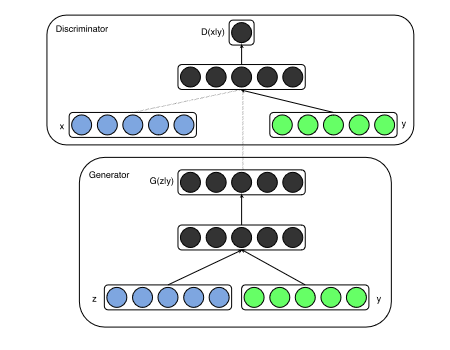
\includegraphics[width=0.5\textwidth]{cgan.png}
	\caption{Conditional Adverserial Network}
	\label{fig:Bild38}
\end{figure}

\subsection{3D-GAN}\label{sec:3dgan}

Das besondere am 3D Raum im Vergleich zu normalen 2D Bildern ist die Steigerung der Dimension und zu gleich der hohe Informationsgehalt welcher in 3D Objekten steckt. Das Ziel von 3D-GAN ist es die Datenverteilung der zugrunde liegenden 3D-Modellen zu erlernen. Dabei wird der latente Objektraum erfasst und soll dadurch die Wahrscheinlichkeiten für einzelne Objektklassen enthalten. 
\\\\
Es wurden schon mehrere Versuche von generativen Modellen auf 3D Daten durchgeführt wie von Wu, Jiajun und Zhang \cite{3d} welche in ihren Modell mit mit 3D-Voxel Daten arbeiten und damit ein GAN trainiert haben.Auch Achlioptas, Panos und Diamanti\cite{3dgan} welche ein GAN auf Punktwolken trainiert. Da in folgender Arbeit die 3D-Daten durch Punktwolken dargestellt werden wird die Arbeit von Achlioptas, Panos und Diamanti näher beleuchtet.
\\\\
Die Architektur des typischen 3D-GAN oder auch RAW-GAN betitelt ist dem Vanilla GAN von Goodfellow ähnlich. Der Input Layer ist ein Fully-Connected Layer welcher der Anzahl der Punkte je Punktwolke * 3 entspricht. Dieser bekommt als Input einen Noise-Vektor welcher aus einer Normal Verteilung entnommen wird und durch mehrere Layern gereicht bis hin zum Output Layer welche die Anzahl der gewünschten Punkte besteht. Also Zielfunktion kann mit der KL-Zielfunktion gearbeitet werden oder mit der Wasserstein Metrik welche im Versuchsaufbau von Achlioptas, Panos und Diamanti besser Ergebnissee geliefert hat. Der Aufbau unterscheidet sich nicht von Vanilla-GAN\cite{3dgan}. 

\begin{figure}[htbp] 
	\centering
	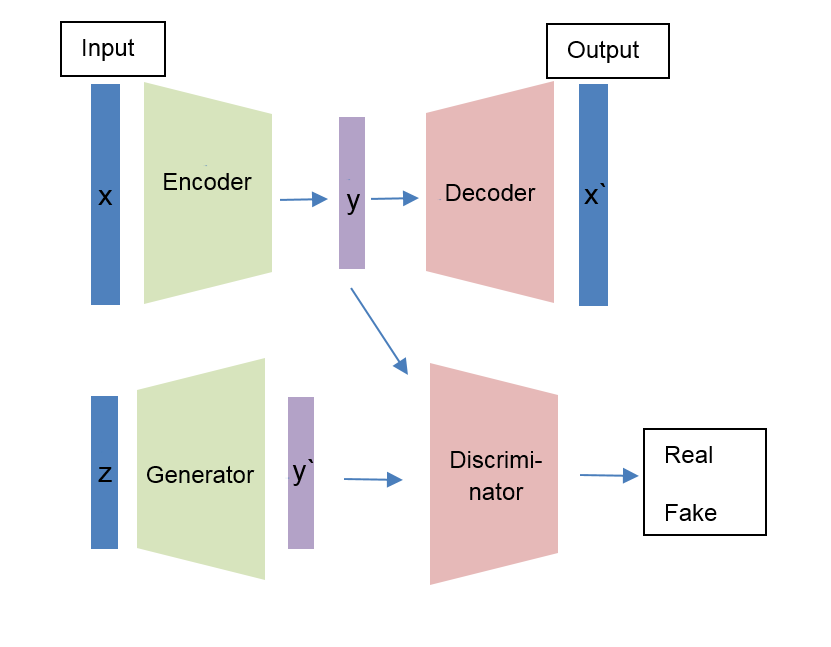
\includegraphics[width=0.5\textwidth]{latentgan.png}
	\caption{Latent-GAN}
	\label{fig:Bild39}
\end{figure}
~\\\\
Eine weitere Möglichkeit ist das Latent-GAN, dieses benutzt eine andere Aufbau gegenüber dem RAW-GAN, welches dabei helfen soll den latenten Raum der Objekte zu erlernen. Zunächst wird ein Autoencoder mit den vorhanden Trainingsdaten(vgl. \ref{sec:autoencoder}) trainiert. Der Aufbau ist der selbe einen üblichen 3D-Autoencoder beschrieben in Kapitel \ref{sec:autoencoder}. Ziel dabei ist den latenten Raum der Trainingsdaten zu erlernen und eine Kompression der Daten um den Suchraum zu  welcher beim RAW-GAN durch die Inputdimension gegeben ist, zu verringern und dadurch das Training des GANs zu erleichtern\cite{3dgan}. 
\\\\
Bevor das Training des Latent-GAN beginnen kann werden nun die Trainingsdaten durch den vorher trainierten Encoder des 3D-Autoencoder auf die festgelegte Output-Dimension komprimiert. Anschließend werden diese komprimierten Daten verwendet um das GAN zu trainierten. Dabei erlernt das GAN komprimierten Code zu produzieren, welcher anschließend durch den Decoder des 3D-Autoencoder wieder auf die ursprüngliche Größe gebracht werden kann. Durch dieses Verfahren war es möglich Daten in einer guten Qualität zu produzieren und eine Datenverteilung des zugrundeliegenden Models zu erlernen. Der gesamte Ablauf kann in \ref{fig:Bild39} entnommen werden\cite{3dgan}. 

\subsection{Rekonstruktion von Daten}\label{sec:rekdaten}

Derzeit setzt Deep Learning neue Maßstäbe bei der Rekonstruktion von Daten, wie Bildern oder Texten. Bei der Rekonstruktion geht es darum Daten, welche von ihren Urzustand verändert wurden, sei es durch Artefakte oder manuelle Bearbeitung, wieder dahin zurück geführt werden. In Abb. \ref{fig:Bild40} ist eine Rekonstruktion eines Bildes dargestellt welches eine Wiederherstellung eines Hundes zeigt. Deep Learning hat in diesem Bereich besonders bei Bilder große Erfolge erzielt. Da diese als Matrizen dargestellt werden können, liefern sie eine Datenstruktur, auf welche KNN arbeiten können. Auch Bearbeitung mit Convolutionen-Layer auf Bilddaten zählt als Erfolg für die Weiterverarbeitung\cite{imagerecon}. Durch die genannten Methoden werden bessere Strukturen für das jeweilige Ziel, in diesem Fall die Rekonstruktion, gelernt und ermöglicht es wie in verschieden Papern wie \cite{imagere1}  welche auf super-hochauflösenden Bildern Artefakte entfernt und das Bild wieder zum Urzustand zurück führt.
\\\\
Auch wie die Arbeit von Liu, Gulin und Reda \cite{imagere2} konnte ähnliche Ergebnisse liefern. Rekonstruktion auf 3D-Daten wurde von Yi, Li und Shao \cite{3d_recon} durchgeführt. Diese Arbeiteten beinhaltet jedoch die Rekonstruktion von 2D Bildern auf 3D Modellen. Dabei wurde mit Hilfe von Autoencoder gearbeitet was auch für die folgenden Arbeit von Bedeutung sind\cite{3d_recon}. Da diese helfen durch die Dimensionreduktion eine einfachere Daten Weiterverarbeitung zu liefern. 

\begin{figure}[htbp] 
	\centering
	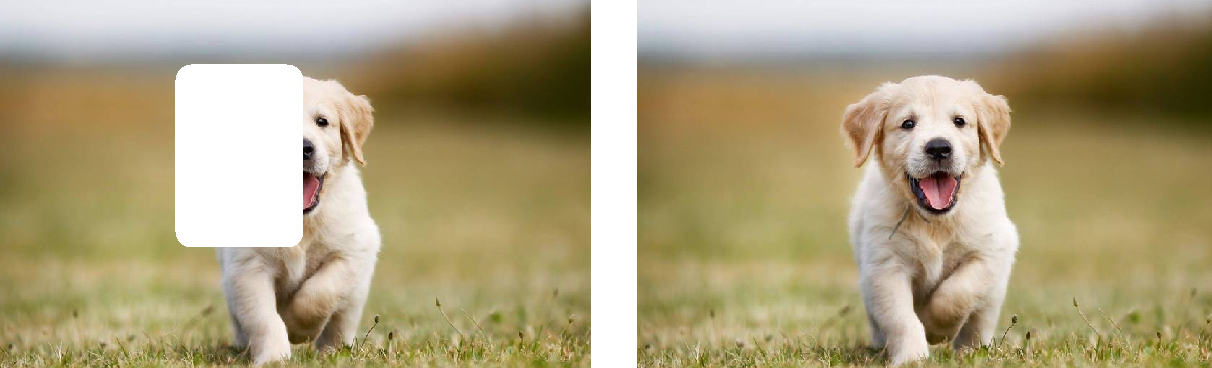
\includegraphics[width=0.6\textwidth]{imagere.png}
	\caption{Bild Rekonstruktion eines Hundes welches durch ein Artefakt zerstört wurde}
	\label{fig:Bild40}
\end{figure}
\newpage
\section{Methoden}
In diesen Kapitel werden die Methoden für die Versuchsaufbauten 1 und 2 aufgezeigt welche die Ziele 1 und 2 überprüfen sollen, diese wurden in \ref{sec:objective} festgehalten.

\begin{description}
	\item[Ziel 1]
	Können durch GANs 3D-Punktwolken von Tabakblättern erlernt werden um neue Datensätze zu generieren?\\
	
	\item[Ziel2] Können durch GANs 3D-Punktwolken von Tabakblättern welche von Tabakblättern von ihren Urzustand abgebracht wurden rekonstruiert werden? 
\end{description}

Dabei geht es darum ob mit Hilfe von GANs der latente Objektraum eines Tabakblattes gelernt werden kann und anschließend durch den Generator des GAN Tabakblätter erzeugt werden können. Dieses Versuchsaufbau wird in Kapitel \ref{sec:versuch1-aufbau} behandelt. Die dazugehörigen Trainingsdaten werden in Kapitel \ref{sec:versuch1-traingsdaten} vorgestellt. Beim Ziel 2 soll überprüft werden ob mit Hilfe von GAN es möglich ist Artefakte von Tabakblätter zu entfernen und den Urzustand wieder her zustellen ist.  Dieses Verfahren wurde in Kapitel \ref{sec:rekdaten} beschrieben. Die Trainingsdaten für diesen Versuchsaufbau können aus Kapitel \ref{sec:versuch2_daten} entnommen werden. 
\\\\
Versuchsaufbau 1.2 und 2.1 wurden auf einen Computer mit Ubuntu 14.05 Betriebssystem mit einen IntelR CoreTM i7-7700k mit 4.50GHz einer Geforce GTX 1080 mit 8G Grafikspeicher. Training und Testen wurden mit CUDA 9.0 und cudNN 7.1.1. Also Programmiersprache wurde Python 2.7 bzw. 3.5 für Datengenerierung. Als ANN Libary wurde Tensorflow 1.5 genutzt und TFlearn 0.3.2. Für die EMD und Chamfer loss für den Autoencoder wurde die Implementierung von  fanqgme (https://github.com/fanhqme/PointSetGeneration) benutzt.
\\\\
Versuchsaufbau 1.1 und 2.2  wurden auf einen Computer mit Windows Betriebssystem mit einen IntelR CoreTM i7-7700k mit 4.50GHz einer Geforce GTX 1080 mit 8G Grafikspeicher. Training und Testen wurden mit CUDA 9.0 und cudNN 7.1.1. Also Programmiersprache wurde Python 3.5 verwendet. Als ANN Libary wurde Tensorflow 1.10 genutzt.


\subsection{Datensatz 1. Versuchsaufbau}\label{sec:versuch1-traingsdaten}
~\\\\
Der erste Datensatz "Stühle" besteht aus 6778 Punktwolken mit je 2048 Punkten. Dieser wurde aus den Shapenet Datensatz(www.shapenet.org) entnommen. Die Daten sind PLY Datenformat abgespeichert. Ein Beispielpunktwolke kann aus Abbildung entnommen werden. Der Datensatz wurde in der Arbeit von Achlioptas, Diamanti, Mitliagkas und Guibas\cite{3dgan} verwendet welches auch in Kapitel \ref{sec:3dgan} vorgestellt wurde ist. In dieser Arbeit dient er als Validierungsdatensatz um die Qualität der generierten Daten des GAN welches mit Tabakblättern trainiert wurde zu vergleichen.
\\\\
Die Daten für den zweiten Datensatz Blätter stammen vom Fraunhofer Institut deren Gewinnung wurde in Kapitel \ref{sec:punktwolken} beschrieben. Der Grunddatensatz bestand aus mehreren 3D-Scans von Tabakpflanzen bei den die Blätter der Pflanze zu einen Datensatz zusammengefügt wurden sind. Der Blätter Datensatz besteht aus 422 Punktwolken welche dann durch ein Punktreduktionsverfahren auf jeweils 2048 Punkten je Punktwolke reduziert wurden ist. Aus Komplexitätsgründen wurden der Farbchannel außen vor gehalten um den Informationsgehalt der Daten zu reduzieren und ein Training zu vereinfachen. Außerdem spielen Farben bei den derzeitigen Ziel der Arbeit, Rekonstruktion von Tabakblättern keine Rolle und nehmen keinen Einfluss auf die Verwendbarkeit des Ergebnisses. Abgespeichert werden die Daten im .ply Datenformat.

\begin{figure}[htbp] 
	\centering
	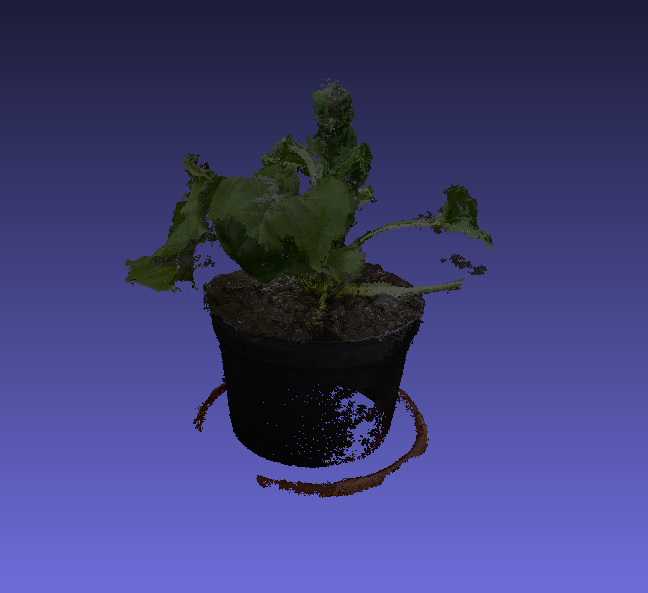
\includegraphics[width=0.5\textwidth]{plant.png}
	\caption{3D Punktwolke einer Tabakpflanze}
	\label{fig:Bild50}
\end{figure}

\begin{figure}[htbp] 
	\centering
	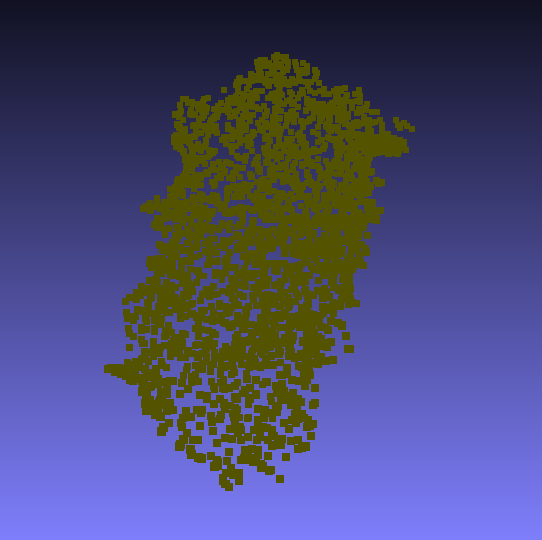
\includegraphics[width=0.5\textwidth]{leaf1.png}
	\caption{3D Punktwolke einer Tabakpflanze}
	\label{fig:Bild51}
\end{figure}
\newpage
\subsection{Datensatz 2. Versuchsaufbau}\label{sec:versuch2_daten}

Für den zweiten Versuchsaufbau wird auf den in Datensatz Versuchsaufbau 1. Blatt Datensatz "Blätter" zurück gegriffen. Das heißt der Grunddatensatz besteht aus 422 unterschiedlichen Blättern. Dieser Datensatz wird nun dahingehen verändert um das Rekonstruieren von Tabakblättern welche durch Artefakte von ihren Urzustand verändert wurden Rückgengig zu machen. Die Artefakte simulieren dabei das Verdecken von anderen Blättern beim Scanverfahren was zu unvollständigen Blättern führen kann. Dieses verdecken wir durch 3D-Sphären simuliert wie in Abb. \ref{fig52} dargestellt. Die Sphären bestehen aus 100 000 Punkte welche alle einen maximalen Radius von 15 mm haben und welcher jeder Punkt aus einer Normalverteilung entnommen wird um  eine gleichmäßige Verteilung der Punkte zu gewährleisten. Die Sphären werden nun vom Koordinatenursprung in euklidischen Raum bewegt das sich 46 unterschiedlichen Sphären im Raum ergeben. Diese werden dahin gehen Bewegt um möglichst eine hohe Differenzmenge mit den 422 Blättern im Datensatz zu haben. In Abb  \ref{fig:Bild52} sind alle Sphären symbolisch eingefügt werden um dieses Vorgehen zu Veranschaulichen. Um nun das Verdecken zu Simulieren wird die Differenzmenge je Blatt mit einer der Sphären genommen. Wobei die Differenzmenge eines Punktes der nähst Nachbar in einen Radius von 3mm befindet. Durch die dieses Verfahren entstehen Kreisförmige Löcher in den Blättern welches in Abb. \ref{fig:54} dargestellt ist. Anschließend werden alle erzeugten "zerstörten" Blätter nach der Anzahl ihrer übrig geblieben Punkte gefiltert um zu gewährleisten das genügen Punkte aus dem Urblatt entfernt wurden sind und eine visuelle Diskrepanz zwischen den Blätter vorhanden sind. Was letztendlich zu 2047 zerstörten Blättern geführt hat mit jeweils 2048 Punkten.

\begin{figure}[htbp] 
	\centering
	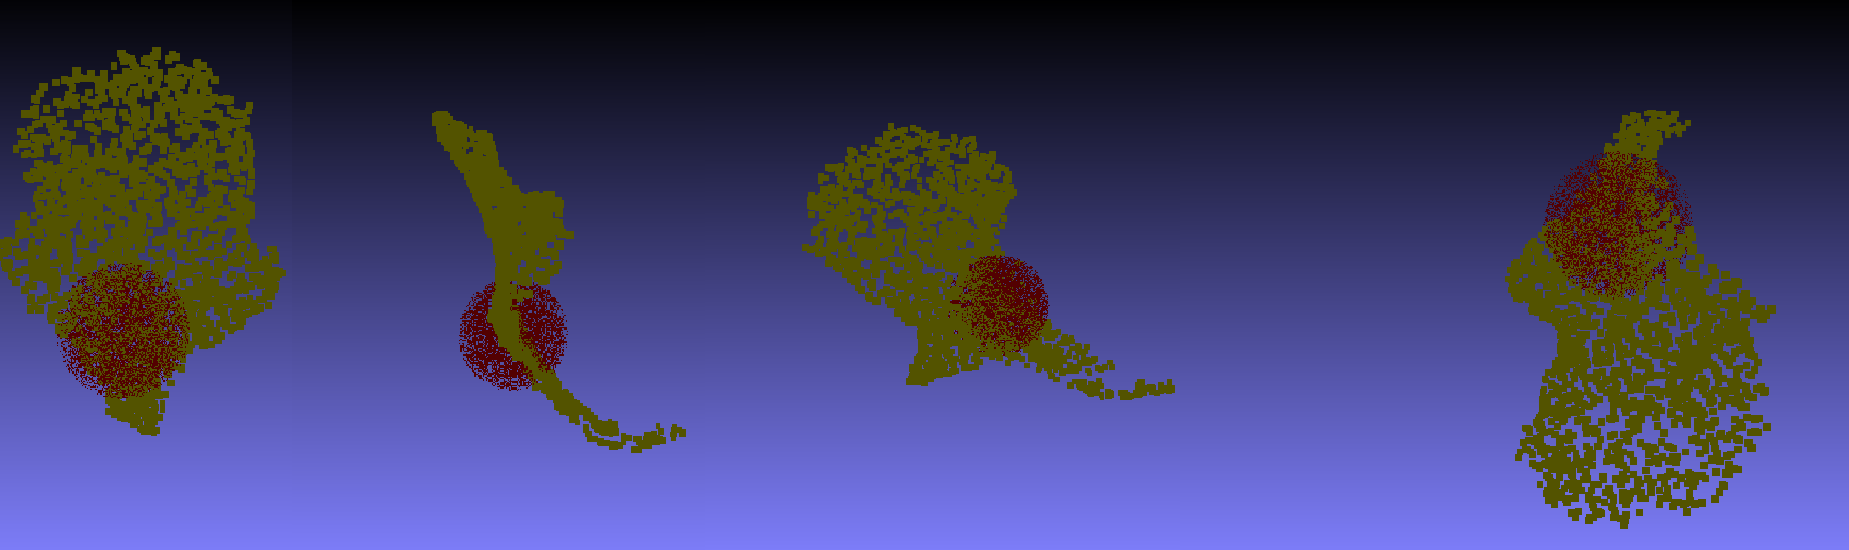
\includegraphics[width=1.0\textwidth]{sphere1.png}
	\caption{Tabakblatt mit Sphäre welche die Differenzmenge bilden}
	\label{fig:Bild52}
\end{figure}

\begin{figure}[htbp] 
	\centering
	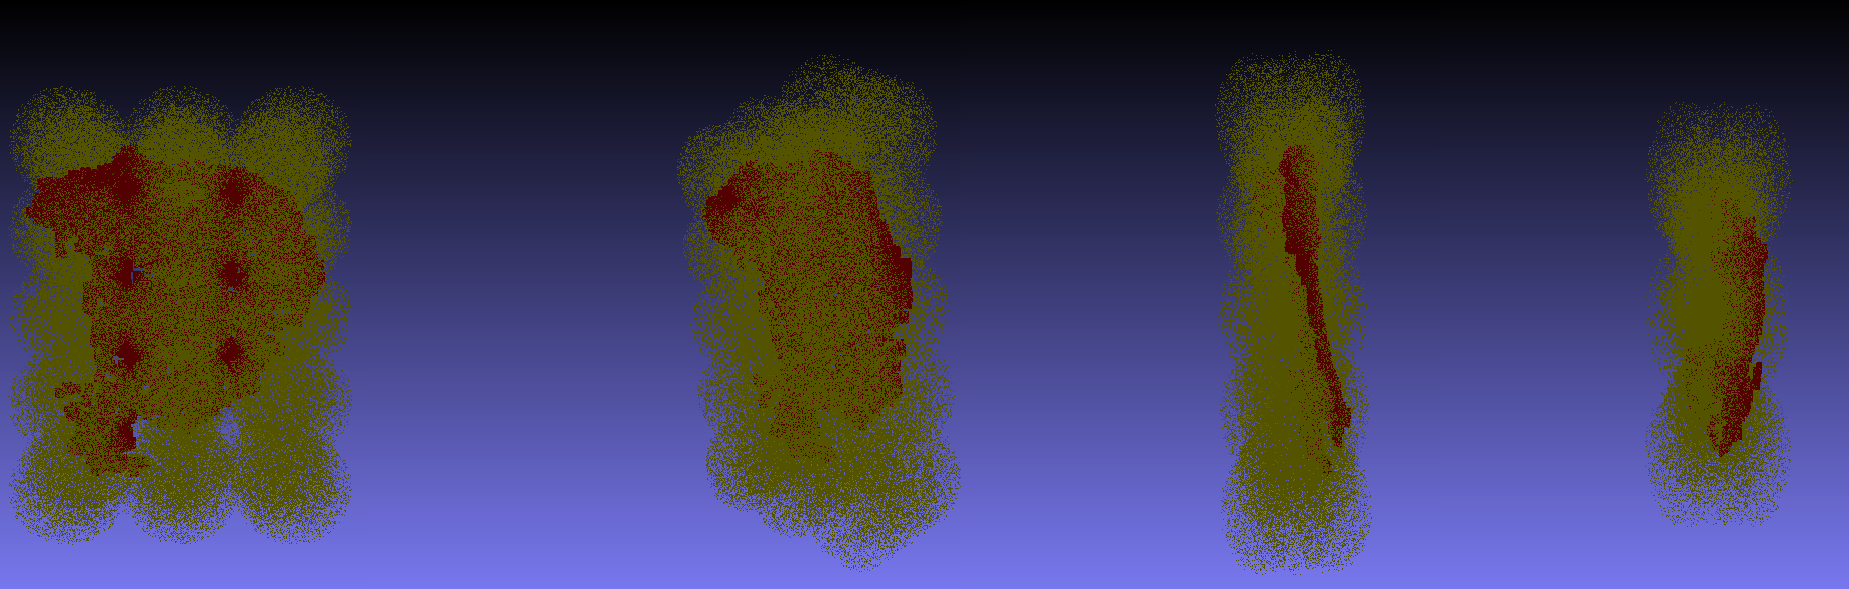
\includegraphics[width=1.0\textwidth]{allsphere.png}
	\caption{Sphäre im Raum welche das verdecken der Blätter simulieren}
	\label{fig:Bild53}
\end{figure}

\begin{figure}[htbp] 
	\centering
	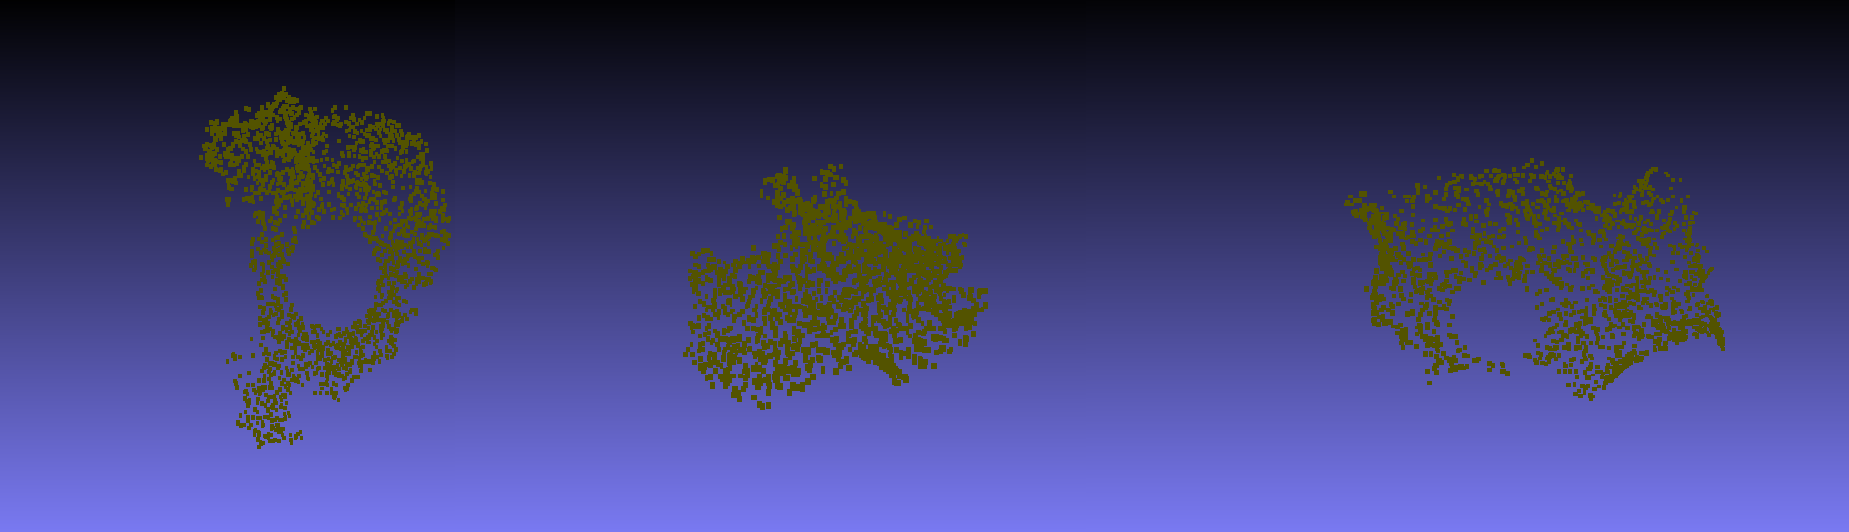
\includegraphics[width=1.0\textwidth]{training_destroyed.png}
	\caption{3D Punktwolke einer Tabakpflanze}
	\label{fig:Bild54}
\end{figure}
\newpage


\subsection{Versuchsaufbau 1 - GAN}\label{sec:versuch1-aufbau}

Der Versuchsaufbau 1 besteht aus zwei unterschiedlichen Versuchen. Aufbau 1.1 ist das RAW-GAN(\cite{3dgan}), dabei wird auf den Vanilla-GAN Aufbau zurückgegriffen. Die Meta Trainingsvariablen für diesen Versuch sind Learningrate mit 0,0005 und einen Adam Optimizer welcher zu den stochastischen Gradient Descent Verfahren aus Kapitel \ref{sec:test} und dabei auf das aus Kapitel \ref{sec:momentum} zurückgreift, mit einem Beta1 von 0,5 und einem Beta2 von 0,5. Die Batchgröße ist 64. Der Discriminator besteht aus 5-Layern welche aus 1-Dimensionalen Convolutionen-Layer bestehen mit einer Filteranzahl [64, 128, 256, 256, 512] je Layer. Mit einer Kernel Größe von 1 und Stride von 1. Also Aktivierungsfunktion wird die ReLu-Funktion genutzt. Darauf folgen 3 Fully-Connected-Layer mit der Größe [128, 64, 1] alle mit einer ReLu-Funktion. Der Generator des RAW-GAN besteht auf 6 Fully-Connected-Layern mit [64, 128, 512, 1024 ,1536 ,6144] Neuronen, jeweils mit der Relu Aktivierungsfunktion. Der Noisevektor z wird aus einer 128-D Normal Verteilung entnommen mit $\mu$ = 0 und $\sigma$ =  0,2. Als Zielfunktion wird die Wasserstein Metric gewählt da diese bessere Ergebnisse im Versuchsaufbau von Achlioptas, Panos und Diamanti\cite{3dgan} erzielt hat. Das Training erfolgt jeweils mit den Datensätze "Stuhl" und "Tabakblätter" beschrieben in Kapitel \ref{sec:versuch1-traingsdaten}.
\\\\
Der Versuchsaufbau 1.2 ist das Latent-GAN welches in Kapitel \ref{sec:3dgan} vorgestellt wurde. Es wurde die Implementierung von \cite{3dgan} verwendet $(www.github.com/optas/latent_3d_points)$. Zunächst wird dabei der Autoencoder mit den Trainingsdaten trainiert. Das Training erfolgt einer Learningrate von 0,0005 und einer Batchsize von 50. Der Encoder besteht dabei aus 4 1-D Convolutional-Layern mit [64, 128, 246, 1024] Filtern, eine Stride von 1 und Size von 1. Die Batchgröße ist 64. Als Aktivierungsfunktion wir die Relu verwendet. Der Encoder besteht aus 3 Fully-Connected-Layern mit [256, 256, 6144] Neuronen, alle mit der ReLu-Zielfunktion. Das Training erfolgt jeweils mit den Datensätze "Stuhl" und "Tabakblätter" beschrieben in Kapitel \ref{sec:versuch1-traingsdaten} und wurde auf 500 Epochen durchgeführt. 
\\\\
Nach dem Training des Autoencoder kann der komprimierte Latent Code welcher von Encoder erstellt wird dazu verwendet werden das Latent-GAN zu trainieren. Alle Trainingsdaten werden nun durch den Encoder komprimiert um ihre 128-D Latenten Code y zu erzeugen. Mit diesen wird nun das GAN trainiert um eigene Latente Code zu produzieren welche von den Decoder wieder auf ihre ursprüngliche Dimension von 2048 Punkten zu projizieren. In Abb. \ref{fig:Bild39} ist dieser Prozess dargestellt. Der Generator des Latent-GAN besteht aus 2 Fully-Connected-Layer mit [128, 128] Neuronen welche als Aktivierungsfunktion eine ReLu-Funktion benutzen. Der Noisevektor z wird aus einer 128-D Normal Verteilung entnommen mit $\mu$ = 0 und $\sigma$ =  0,2. Der Discriminator besteht aus [128, 64, 1] Fully-Connected-Layern welche ebenfalls ReLu-Funktion nutzen.Als Zielfunktion wird die Wasserstein Metrik gewählt da diese bessere Ergebnisse im Versuchsaufbau von Achlioptas, Panos und Diamanti\cite{3dgan} erzielt hat. 

\subsection{Versuchsaufbau 2 - CGAN für Punktwolkenrekonstruktion }\label{sec:versuch2-aufbau}

Da sich im Versuchsaufbau 1 das Latent-CGAN bessere Ergebnisse liefert bei erlernen von Punktwolken Daten. Wird im Versuchsaufbau 2.1 Latent-CGAN das komprimieren von Trainingsdaten übernommen und dahin gehen verändert, das Ziel von C-GAN zu übernehmen und bedingte Wahrscheinlichkeiten zu lernen. Zunächst werden wie bei Versuchsaufbau 1 die Trainingsdaten vgl.\ref{sec:versuch1-traingsdaten} an einen Autoencoder trainiert. Dabei wird jeweils ein Autoencoder für zerstörte Blätter heran genommen und einer für unzerstörte im Urzustand befindende Blätter.
\\\\
Die Autoencoder folgen dabei den gleichen Aufbau wie in Versuchsaufbau 1.2. Der Encoder besteht dabei aus 4 1-D Convolutional-Layern mit [64, 128, 246, 1024] Filtern, eine Stride von 1 und Size von 1. Als Aktivierungsfunktion wir die Relu verwendet. Der Decoder besteht aus 3 Fully-Connected-Layern mit [256, 256, 6144] Neuronen, alle mit der ReLu-Zielfunktion. Als Batchsize wird 64 genommen. Als Zielfunktion wird jeweils einmal die Chamfer Distance getestet und die Earthmover Distance. Für den Autoencoder wurde die Implementierung von \cite{3dgan} verwendet $(www.github.com/optas/latent_3d_points)$ 
\\\\
Der Generator des Latent-CGAN bekommt als Input z einen 128-D Vektor, welcher aus einer Normal Verteilung entnommen mit $\mu$ = 0 und $\sigma$ =  0,2. Y welches zusätzlich zu z den Generator zum Training eingespeist wird sind die von Autoencoder codierten 128-D komprimierten "zerstörte" Tabakblätter. Der Generator des Latent-GAN besteht aus 2-Fully-Connected-Layer mit [128, 128] Neuronen welche als Aktivierungsfunktion eine Leaky-ReLu-Funktion benutzen. Der Discriminator besteht aus 2 Fully-Connectected-Layern mit der Größe [128, 128]. Der Discriminator bekommt als Input entweder den vom Generator erzeugten latenten Code x' welcher vom Encoder des Autoencoder zu einen unzerstörten Blatt gemappt werden kann und zusätzlich y also (x`,y). Oder ein aus unseren Trainingsdaten stammendes (x,y) Paar welches als reale-Datensätze gekennzeichnet ist. Als Ziel wird jeweils das Wasserstein Metrik und die Vanilla - GAN Metrik Loss-Function benutzt.
\\\\
Beim Trainingsaufbau 2.2 RAW-CGAN bekommt der Generator als Input Noisevektor z einen 128-D Vektor aus einer  Normal Verteilung entnommen mit $\mu$ =  0 und $\sigma$ =  0,2. Des weiteren wird als y den Generator die  zerstörte Blatt Punktwolken welche als ein 6144-D Vektor dargestellt werden als Input übergeben. Der Generator besteht aus Fully-Connected-Layern mit [6272, 3163, 1568, 3136, 4850, 5680, 6144] Neuronen je Layer. Als Aktivierungsfunktion wird die Leaky-ReLu genommen. Im letzten Layern wird keine Aktivierungsfunktion verwendet um den Output linear Verarbeitbar zu machen und damit Euklidische Koordinaten generiert werden können. Des weiteren wird nach jedem Layer ein Batch-Normalisation-Layer eingesetzt mit Momentum 0,9 und einen Beta1 und Beta2 von 0,5 eingesetzt. Des Discriminator besteht aus [12288, 6144, 3072,1536, 768, 384, 128, 32, 1] Fully-Connected-Layern mit Aktivierungsfunktion Leaky-ReLu bis auf den letzten Layer in den wird die Sigmoid-Funktion verwendet, wenn als Zielfunktion die Vanilla-GAN gewählt wird. Bei Verwendung der Wasserstein Metrik wird auf eine Aktivierungsfunktion verzichtet. Des weiteren wird nach jedem Layer ein Batch-Normalisation-Layer eingesetzt mit Momentum 0.9 und einen Beta1 und Beta2 von 0,5. Der Input des Discriminator sind die von Generator erstellten (x',y) oder die direkt aus dem Trainingsdaten stammenden Punktwolken Paare zerstörtes Blatt y und Urzustand Blatt x als Tupel (x,y).Als Zielfunktion wird die Vanilla-GAN und W-GAN Zielfunktion getestet.
\\\\
Im weiteren Versuchsaufbau für den RAW-CGAN wird der Discriminator umgebaut um ihn durch Convolutional-Layer bessere Lernfähigkeiten geben kann dies sorgt nicht nur für Vorteile für D dadurch kann auch der Generator durch den Gradianten des Discriminators einen besseren latenten Raum lernen soll. Der Generator bleibt in diesen Aufbau gleich der Discriminator bekommt [64, 128, 256, 256, 512] 1-D-Convolutional-Layer mit einer Kernel-Größe von 1 und Stride von 1 als Aktivierungsfunktion wird eine Leaky-ReLu verwendet. Die Batchsize beträgt 64. Anschließend folgen [128, 32, 1] Fully-Conncected Layer mit Leaky-Relu. Zwischen jeden Layer befindet sich ein Batch-Normalisation-Layer mit Momentum von 0,9 und einen Beta1 und Beta2 von 0,5. In Abb. \ref{fig:Bild55} kann der Aufbau und Konnektivät der einzelnen Komponenten entnommen werden.

\begin{figure}[htbp] 
	\centering
	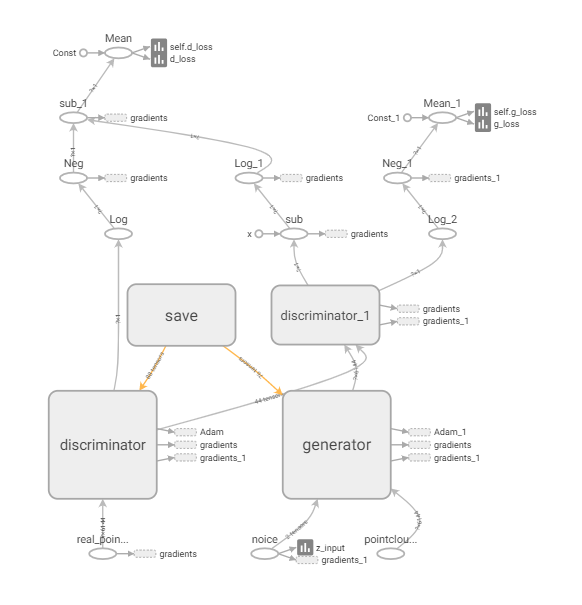
\includegraphics[width=0.6\textwidth]{point-cgan.png}
	\caption{Aufbau des RAW-CGAN}
	\label{fig:Bild55}
\end{figure}
\newpage

\section{Evaluation und Ergebnisse}

Es wird nun in diesen Kapitel auf die Ergebnisse von Versuchsaufbau 1 und 2 eingegangen. Zunächst wird Versuchsaufbau 1 vgl. \ref{sec:versuch1-aufbau} des erlernen von latenten Raum von Punktwolken gezeigt. Dabei wird ein Vergleich zwischen den Modeldaten Satz Stühle sowie einen aus der Praxis Stammenden Datensatz Tabakblätter aufgezeigt. Anschließend wird auf die Ergebnisse aus Versuchsaufbau 2 vgl. \ref{sec:versuch2-aufbau} eingegangen. Dabei wird evaluiert ob es möglich ist die zerstörten Blattdaten auf ihren Urzustand wieder herzustellen und aussagekräftige Ergebnisse für die Anwendbarkeit in der Praxis vorhanden sind. Da es keine gängige Validierungsmethode beziehungsweise Validierungsmetrik gibt wird bei der Prüfung der Testergebnisse auf das menschliche Auge verlassen und die Prüfung erfolgt durch eine Sichtprüfung.  

\subsection{Ergebnisse - Versuchsaufbau 1}

Von RAW-GAN vom Versuchsaufbau 1.1 mit den Blattdaten welches nach 500 Epochen Training lassen sich in Abb.\ref{fig:Bild56} Beispieldatensätze welche vom Generator erzeugten wurden entnehmen. Wie zu erkennen ist sind die Blätter nicht gut genug für eine Weiterverarbeitung. Der Latente Raum welcher von den GAN gelernt wurde und am Ende durch den Generator produziert wurde zeigt keine Ähnlichkeit mit normalen Blättern welche im Datensatz enthalten waren. Die Daten erinnern eher an einen hohlen Ball als an Blättern. Es Formen sich Punktansammlungen nähe des Koordinatenursprungs und es lässt keine Anzeichen von Bilden einer Fläche da. Die Daten erinnern eher an einen hohlen Ball als an Blättern. Wobei eine starke Punkthäufung am Koordinaten Urpsprung festzustellen ist und einzelne verteile Punkte außen herum. Die Starke Punkthäufung am Koordinaten Ursprung ergibt dadurch das die reale Blattdaten an dieser stelle häufig vertreten sind und sich dann an den Blattkanten unterscheiden. Dadurch lernt der Generator an diesen hohen Schnittpunkt mehr Punkte zu generieren als Außerhalb. Dieser Effekt ist in Abb. \ref{fig:Bild81} zu erkennen. Dargestellt sind 24 Datensätze aus den Blattdatensatz welche in einen Koordinaten System geladen wurden sind aus verschiedenen Blickwinkeln. Die Punkte häufen sich in der nähe des Koordinatenursprungs und sind geringer Verteilt im äußeren Bereich. Vergleicht man das nun mit Abb.\ref{Bild56} sind diese dichten Ansammlungen ebenfalls zu erkennen. Der W-GAN Loss für den Generator und Discriminator können in Abbildung \ref{fig:Bild80} entnommen werden. Der Loss des Discriminator und Generator bleibt konstant über mehrere Epochen es ist kein Anzeichen von Verbesserung zu erkennen sollte das Training länger als 500 Epochen laufen. 

\begin{figure}[htbp]
	\centering
	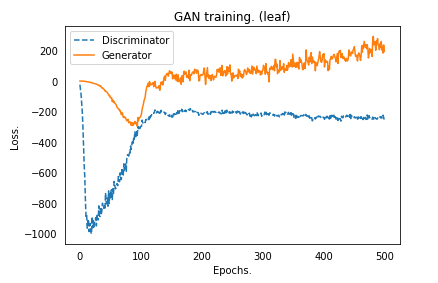
\includegraphics[width=0.5\textwidth]{raw_gan_leaf_result.png}
	\caption{Trainingsverlauf des RAW-GAN mit den Blattdaten}
	\label{fig:Bild80}
\end{figure}
\begin{figure}[htbp] 
	\centering
	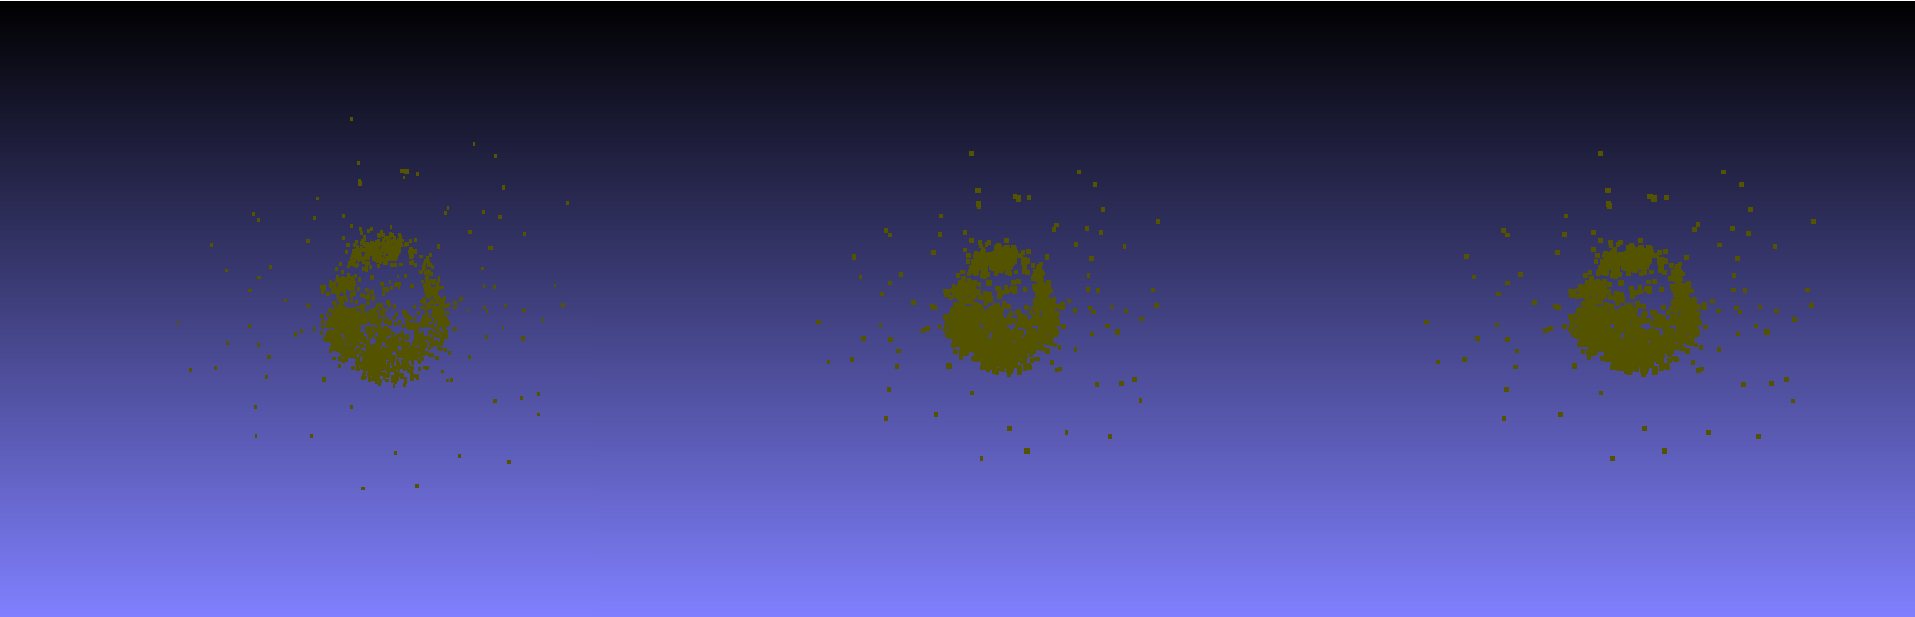
\includegraphics[width=0.5\textwidth]{raw_gan_leaf_example.png}
	\caption{Generierte Beispieldaten von Generator des RAW-GAN mit den Blattdaten}
	\label{fig:Bild56}
\end{figure}
\begin{figure}[htbp] 
	\centering
	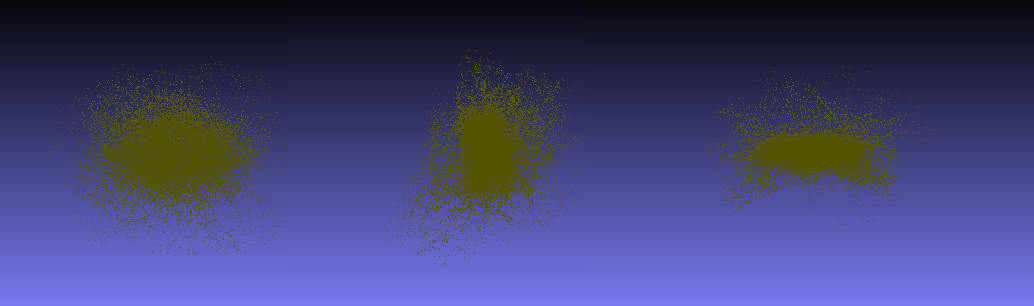
\includegraphics[width=0.5\textwidth]{ansammlung.png}
	\caption{24 Pointclouds aus den Blattdatensatz in einen Koordinatensystem}
	\label{fig:Bild81}
\end{figure}

Ähnliche Ergebnisse sind auch beim RAW-GAN vom Versuchsaufbau 1.1 mit Stuhldaten zu beobachten. Wobei die Qualität der Stühle mehr an die im Trainingsdatensatz stammende Daten erinnert. Es zeichnen sich Lehne und Stuhlbeine von dem GAN trainierten Generator erzeugten Daten ab. Der Trainingsverlauf ist in Abb. \ref{fig:Bild57} zu entnehmen. Dabei ist zu sehen das der Discriminator sich nicht mehr verbessert und der Generator keine besseren Ergebnisse liefern kann. Diese Ergebnisse decken sich mit den von Achlioptas, Panos und Diamanti \cite{3dgan} festgestellten Ergebnissen in den das RAW-GAN keine qualitativ gute Stuhldaten erzeugen konnte. 

\begin{figure}[htbp] 
	\centering
	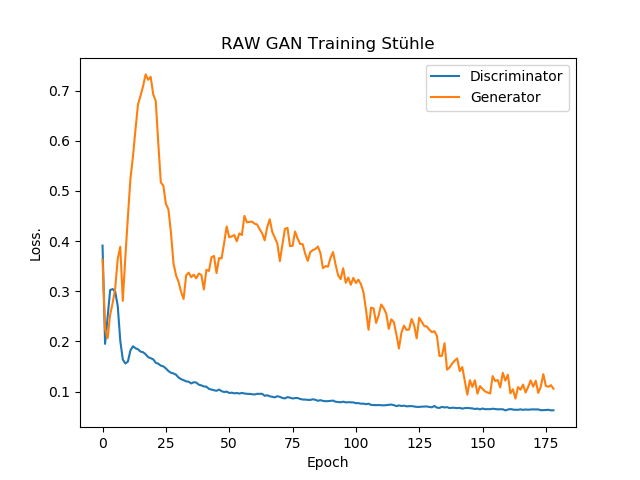
\includegraphics[width=0.5\textwidth]{raw_gan_chair_result.png}
	\caption{Trainingsverlauf des RAW-GAN mit den Stuhldaten}
	\label{fig:Bild57}
\end{figure}

\begin{figure}[htbp] 
	\centering
	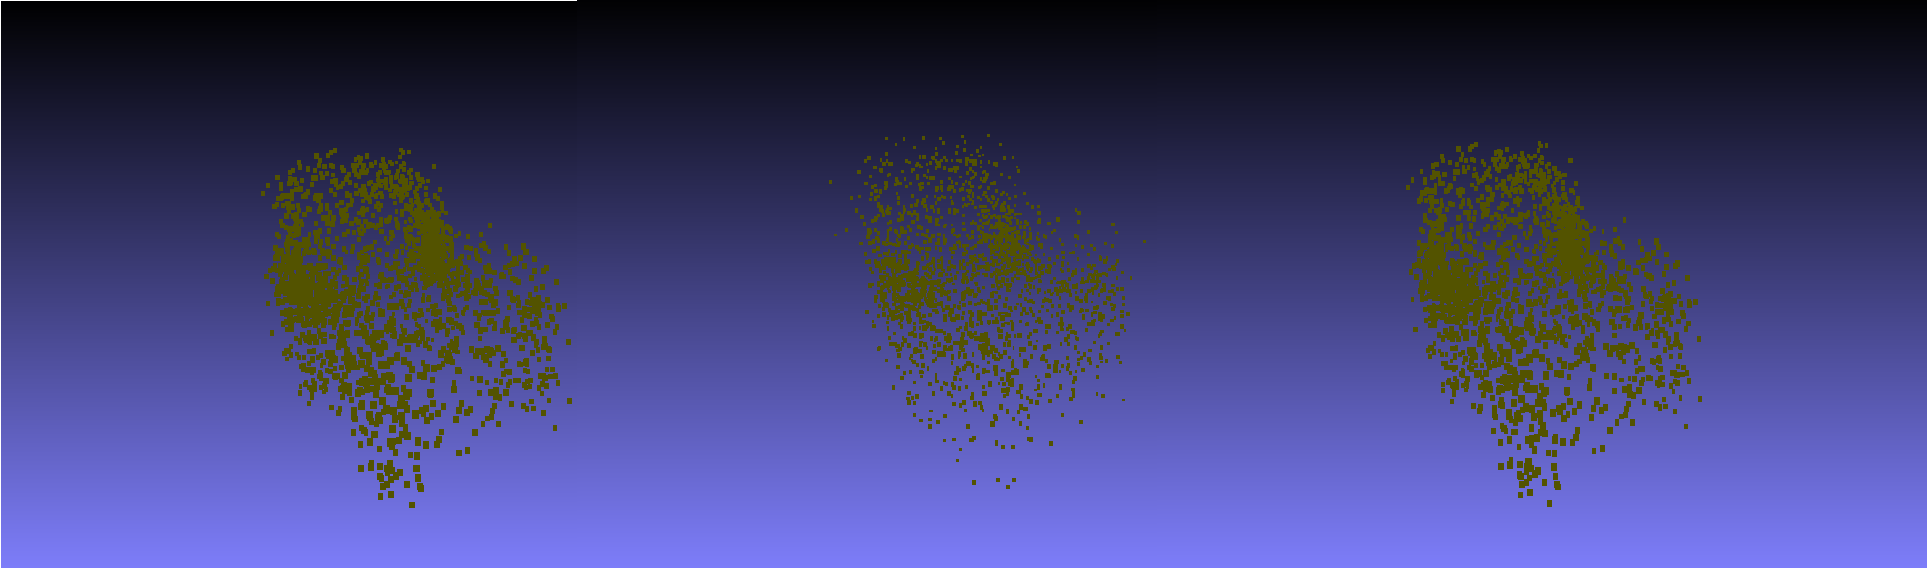
\includegraphics[width=0.5\textwidth]{raw_gan_chair_example.png}
	\caption{Generierte Beispieldaten von Generator des RAW-GAN mit den Stuhldaten}
	\label{fig:Bild58}
\end{figure}

Um nun die Ursache genauer zu begründen, welche die Gründe für  den Qualitätsunterschied zwischen den beiden generierten Daten auszumachen und festzustellen ob durch mehr Blattdaten bessere Ergebnisse erzeugt werden können. Wurden  die Stuhldaten auf 422 Trainingsdaten reduziert und ein erneutes Training des RAW-GAN durchgeführt. Die erzeugte Beispieldaten können aus Abb. \ref{fig:Bild60} entnommen werden. Vergleicht man nun die Qualität von den RAW-GAN mit 422 Stuhldaten Trainingsdaten und 
6778 Stuhldaten  Abb.\ref{fig:Bild59} ist eine Steigerung der Qualität klar festzustellen. Der Trainingsverlauf in Abb. \ref{fig:Bild59} ähnelt der von Abb .\ref{fig:Bild60}. Der Discriminator ist zu schnell perfekt trainiert und gibt den Generator keine Chance mehr nachzuziehen. Es ist eine Tendenz festzustellen das durch eine Erhöhung der Blattdaten auch die Qualität des RAW-GAN steigern könnte.

\begin{figure}[htbp] 
	\centering
	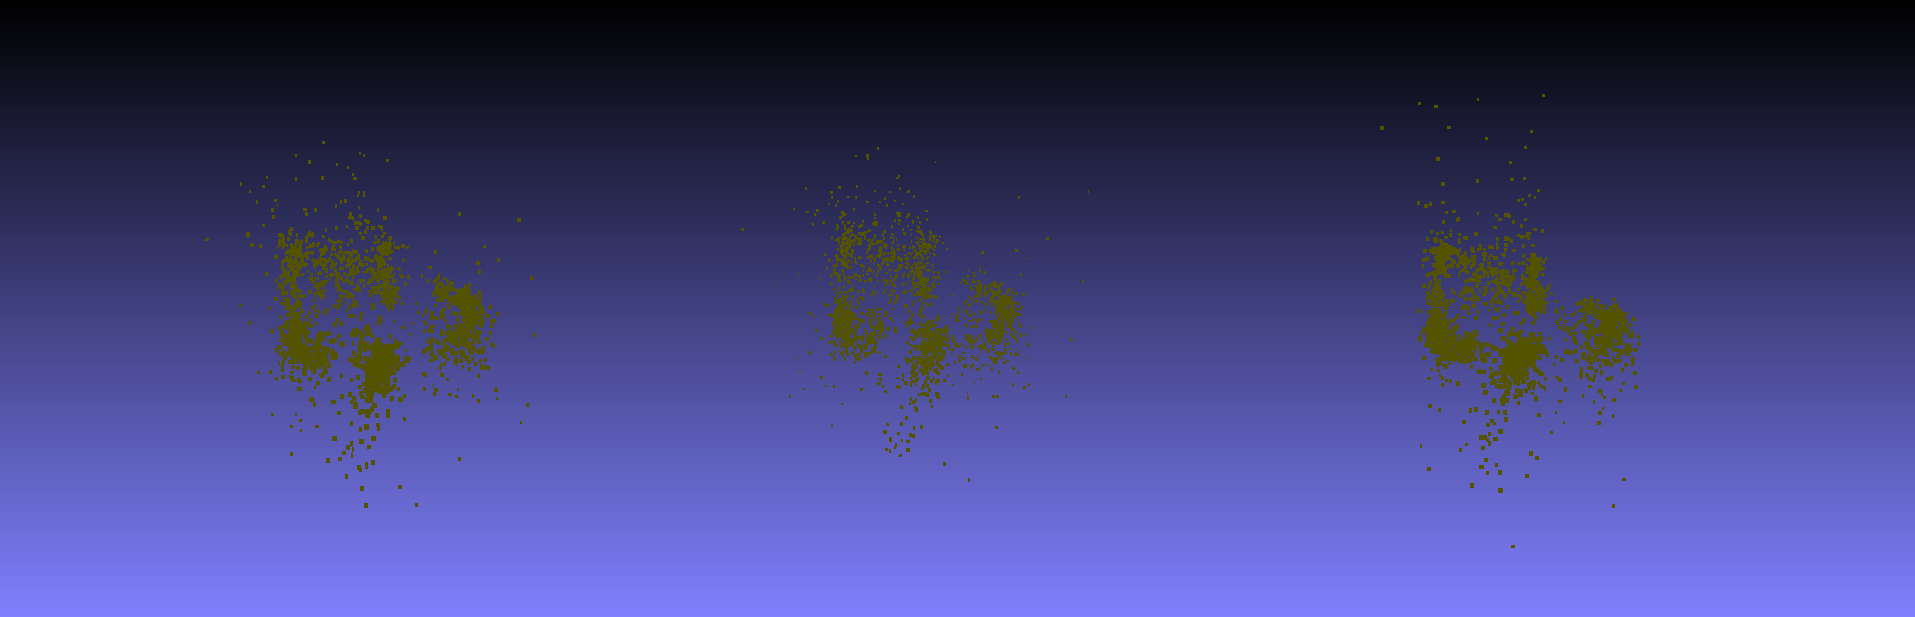
\includegraphics[width=0.5\textwidth]{raw_gan_result_400_result.png}
	\caption{Trainingsbeispiele des RAW-GAN mit den 422 Stuhldaten}
	\label{fig:Bild60}
\end{figure}

\begin{figure}[htbp] 
	\centering
	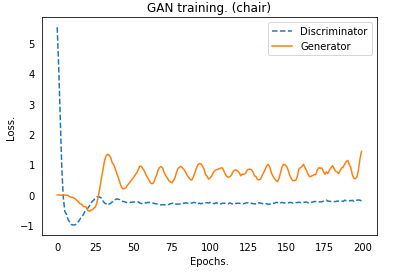
\includegraphics[width=0.5\textwidth]{raw_gan_result_400_examples.png}
	\caption{Trainingsverlauf des RAW-GAN mit den 422 Stuhldaten}
	\label{fig:Bild59}
\end{figure}

Für Versuchsaufbau 1.2 Latent-GAN mit Stühlen kann der Trainingsverlauf aus Abb. \ref{fig:Bild61} entnommen werden. Der Generator Loss verbessert sich zwar gering über mehre Epochen der Discriminator jedoch bleibt konstant auf einen guten Ergebnisse und lässt keine starken Verbesserung des Generators mehr zu. Beispieldatensätze welche von Generator nach Beendigung des Trainings erzeugt wurden in dem der latente-Code von G in den Decoder als Input gegeben wurde sind in Abb. \ref{fig:Bild62} zu entnehmen. Diese sind qualitativ hochwertige Daten welche eine Ähnlichkeit mit denen aus dem Trainingsdatensatz widerspiegeln. Die Ergebnisse decken sich mit den von \cite{3dgan} festgestellten Ergebnissen in den das RAW-GAN keine qualitativ gute Stuhldaten erzeugen konnte. 

\begin{figure}[htbp] 
	\centering
	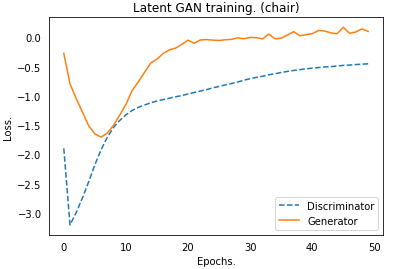
\includegraphics[width=0.5\textwidth]{latent_gan_chair_result.png}
	\caption{Trainingsverlauf des Latent-GAN mit den Stuhldaten}
	\label{fig:Bild61}
\end{figure}

\begin{figure}[htbp] 
	\centering
	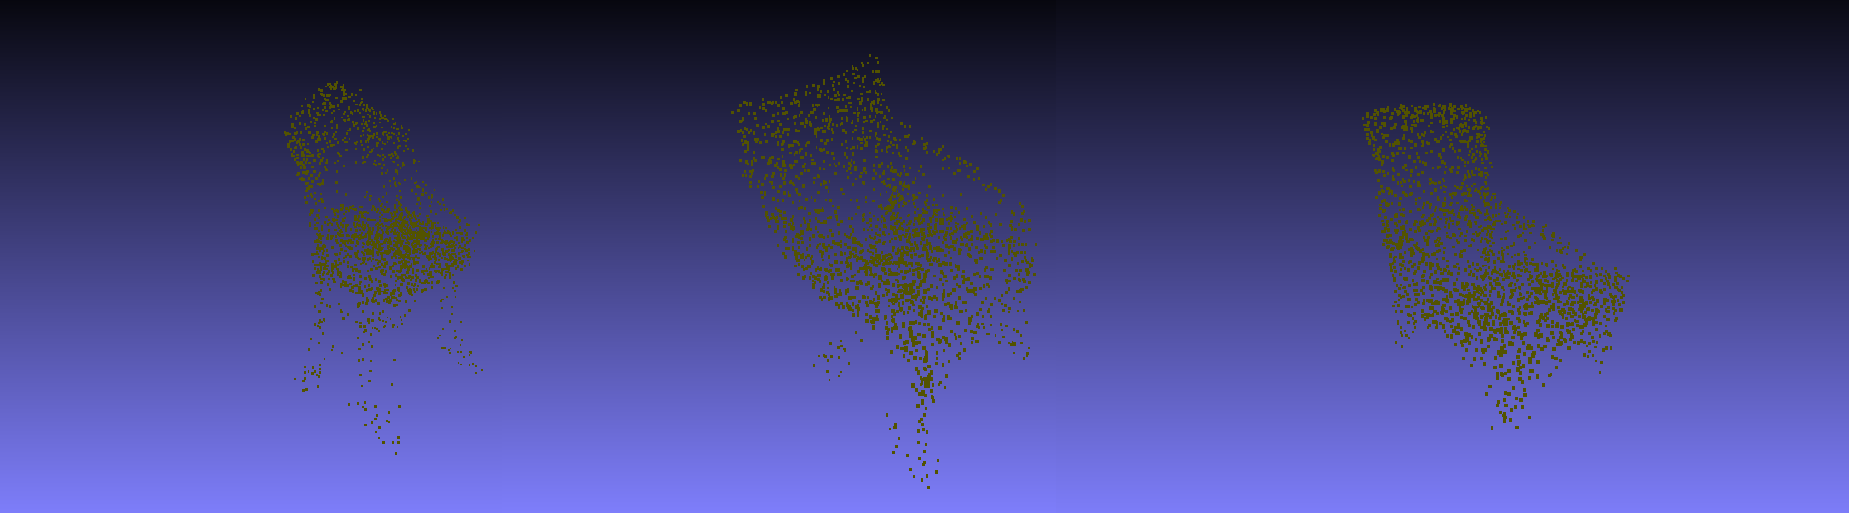
\includegraphics[width=0.5\textwidth]{latent_gan_chair_example.png}
	\caption{Trainingsergebnisse des Latent-GAN mit den Stuhldaten}
	\label{fig:Bild62}
\end{figure}

Das Latent-GAN welches mit den Blattdaten trainiert wurde können exemplarisch generierte Daten aus der Abb. \ref{fig:Bild64} entnommen werden. Diese zeigen eine qualitativ gute Grundfläche welche in der Trainingsdatengesamtheit enthalten ist. Jedoch ist festzustellen das es starke Punkthäufungen an gewissen Bereichen je Blatt gibt, diese sind beispielsweise im 2. Blatt von Rechts in Abb. \ref{fig:Bild64} zu erkennen und mit einen roten Kreis markiert. Der Trainingsverlauf in Abb. \ref{fig:Bild63} zu entnehmen sind keine starken Veränderungen im weiteren Trainingsverlauf zu entnehmen das Training stagniert schon über mehrere Epochen. 
\begin{figure}[htbp] 
	\centering
	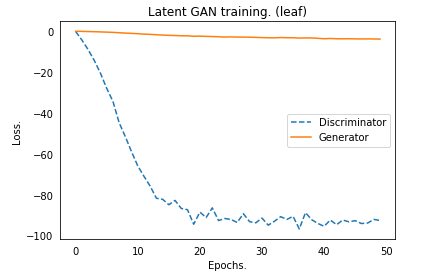
\includegraphics[width=0.5\textwidth]{Latent_gan_training_result.png}
	\caption{Trainingsverlauf des Latent-GAN mit den Blattdaten}
	\label{fig:Bild63}
\end{figure}
\begin{figure}[htbp] 
	\centering
	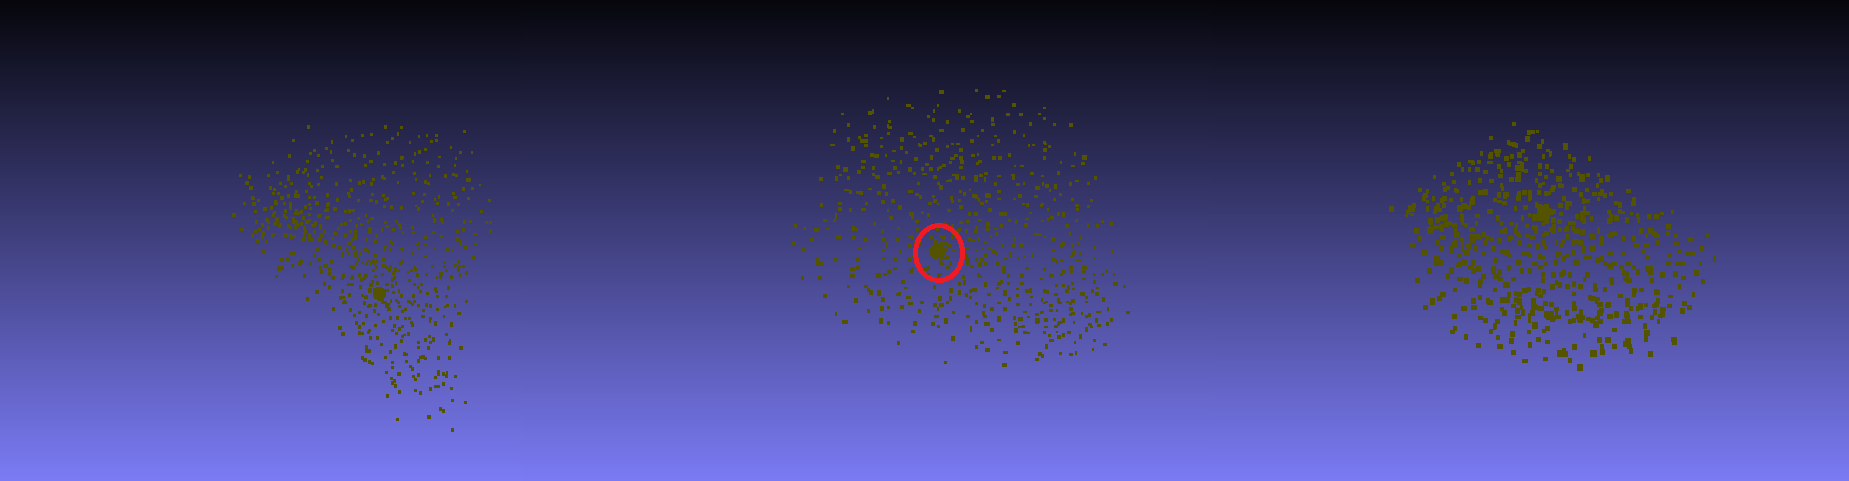
\includegraphics[width=0.5\textwidth]{latent_gan_leaf_example.png}
	\caption{Trainingsergebnisse des Latent-GAN mit den Blattdaten}
	\label{fig:Bild64}
\end{figure}

Um die Ergebnisse von Testaufbau 1.2 Latent-GAN mit Stuhldaten besser zu Vergleichen und um ersichtlich zu machen ob eine Erhöhung der Anzahl der Tabakblätter Daten zu einen besseren Ergebniss führen kann und die Punktanhäufung sich reproduzieren lässt, wurden 422 Stuhldaten genommen um das Latent-GAN zu trainieren. In Abb. \ref{fig:Bild66} sind die exemplarische erzeugte Daten von Generator zu entnehmen. Zu erkennen ist ein ähnlich Phonemen wie bei den Blattdaten. Hohe Punktanhäufungen an Kanten der Sitzfläche zum Übergang der Stuhlbeine. Dadurch lässt sich Rückschlüsse ziehen das eine Erhöhung der Daten zu einer besseren Qualität der Daten führen kann. Der Trainingsverlauf kann aus Abb. \ref{fig:Bild65} entnommen werden auch dieser zeigt eine Stagnation des Verlaufs schon über mehre Epochen an und verspricht keine Erhöhung der Qualität. 

\begin{figure}[htbp] 
	\centering
	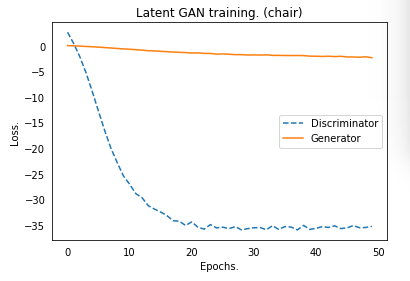
\includegraphics[width=0.5\textwidth]{raw_gan_latent_gan_chair_result_400_example.png}
	\caption{Trainingsverlauf des Latent-GAN mit den Stuhldaten und 400 Trainingsdaten}
	\label{fig:Bild65}
\end{figure}

\begin{figure}[htbp] 
	\centering
	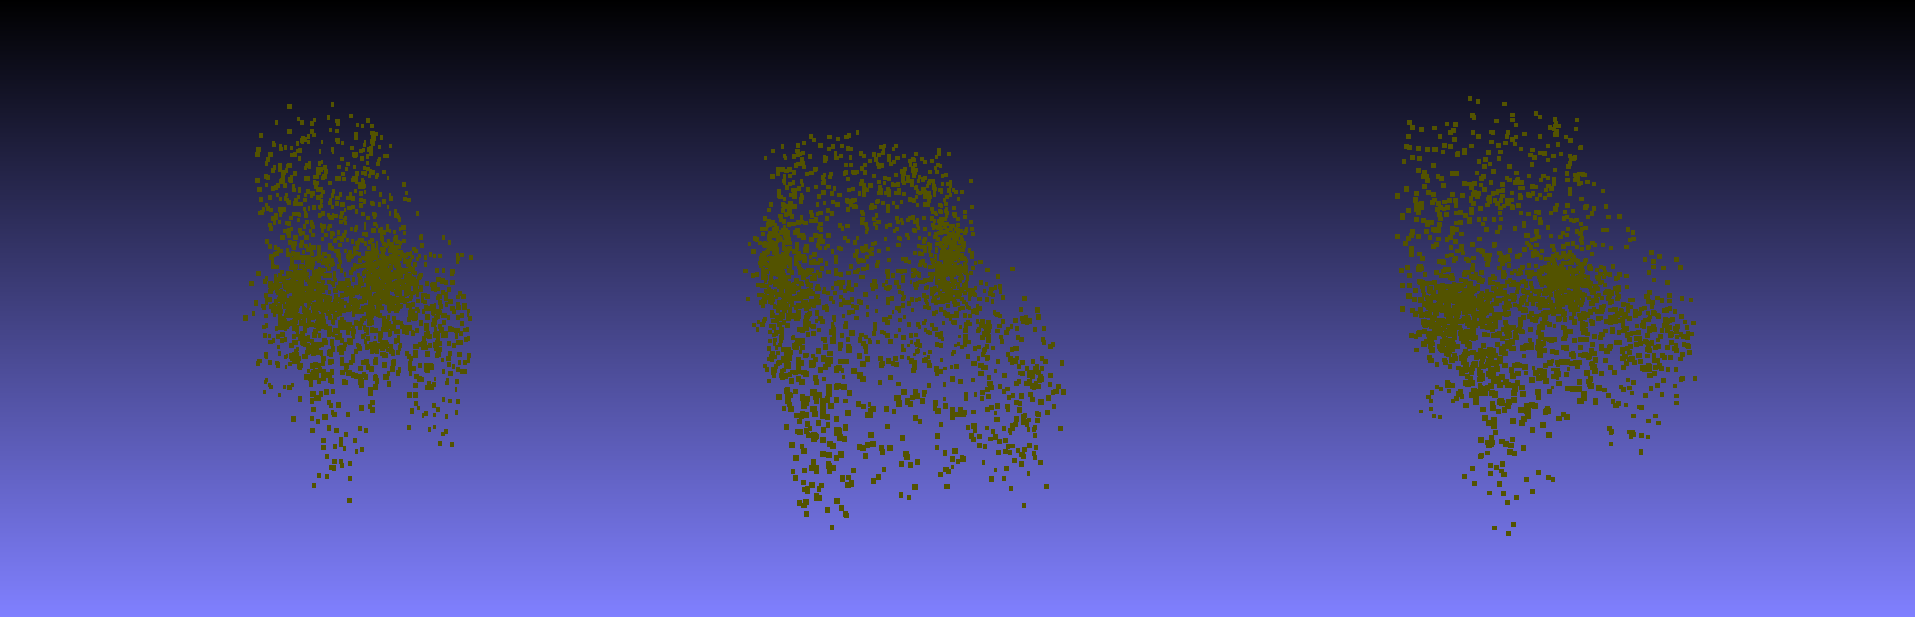
\includegraphics[width=0.5\textwidth]{raw_gan_latent_gan_chair_example_400.png}
	\caption{Traingsergebnisse des Latent-GAN mit den Stuhldaten und 400 Trainingsdaten}
	\label{fig:Bild66}
\end{figure}

Zusammengefasst besonders auf den Hinblick des Blattdatensatzes lässt sich feststellen das bei den Stuhldatensatz die Ergebnisse von Achlioptas, Panos und Diamanti\cite{3dgan} reproduziert werden konnte. Bei einen Datensatz welcher durch Scanverfahren von realen Objekten in diesen Beispiel Tabakblättern konnte gezeigt werden das durch das Latent-GAN eine erste Annäherung an qualitativ Hochwertig generierten Daten zu sehen ist. Durch eine Erhöhung der Trainingsdaten lässt sich auch eine Erhöhung der Qualität feststellen wie bei den Stuhldaten gezeigt wurde, sowie bei RAW-GAN und Latent-GAN. Des weiteren können aber keine Aussagen getroffen werden um welche Höhe die Qualitätssteigerung statt  finden kann. Die Datensätze unterscheiden sich in ihrer Aufbereitung. Die Stuhldaten sind besser auf einen Koordinaten Ursprung geeicht wie in Abb. \ref{fig:Bild85} festzustellen ist, in dieser sind mehre Stühle in ein Koordinaten System geladen zum Vergleich die Blattdaten im Abb. \ref{fig:Bild81} Zu erkennen ist einen enorme Überschneidung der einzelnen Punktwolken bei Stühlen im Vergleich zu Blattdaten dies hilft den Suchraum für die GANS einzuschränken und erleichtert das Training. Es müssten sich bessere Datenvorverarbeitungsschritte bei den Blattdaten erhoben werden. Außerdem sind die 422 Blattdaten zum Vergleich zu den 6778 Stuhldaten sehr gering und hilft den Latenten-GAN und RAW-GAN den latenten Raum besser zu erlernen da die Grundgesamtheit mehr abgedeckt ist. Aus technischer Sicht könnte bessere Layer strukturen für bessere Ergebnisse. Die Bearbeitung mit Convolutionen-Layer auf Bilddaten hat erst den großen Durchbruch bei der Rekonstruktion bei Bilddaten möglich gemacht\cite{imagerecon}. Da nun unser Generator nur aus Fully-Connected-Layern besteht und 3D-Punktwolken komplexer sind als Bilder kann an dieser Stelle definitiv noch nachgearbeitet werden. Beispielsweise könnte ein 1D-Deconvolutional-Layer implementiert werden. Welche bei Tensorflow 1.12 als Prototyp zur Verfügung steht. Eine andere Möglichkeit wäre auf die Arbeit von Cai, Zhongang  und Yu \cite{3d-conv} anzusetzen dieser postuliert eine Methode für 3D-Convolution Methode welche auf 3D-Punktwolken arbeitet und eine Invarianz im Euklidischen Raum lernt mit deren Hilfe es leicht sein soll Rotationen der Punktwolke zu erlernen.

\begin{figure}[htbp] 
	\centering
	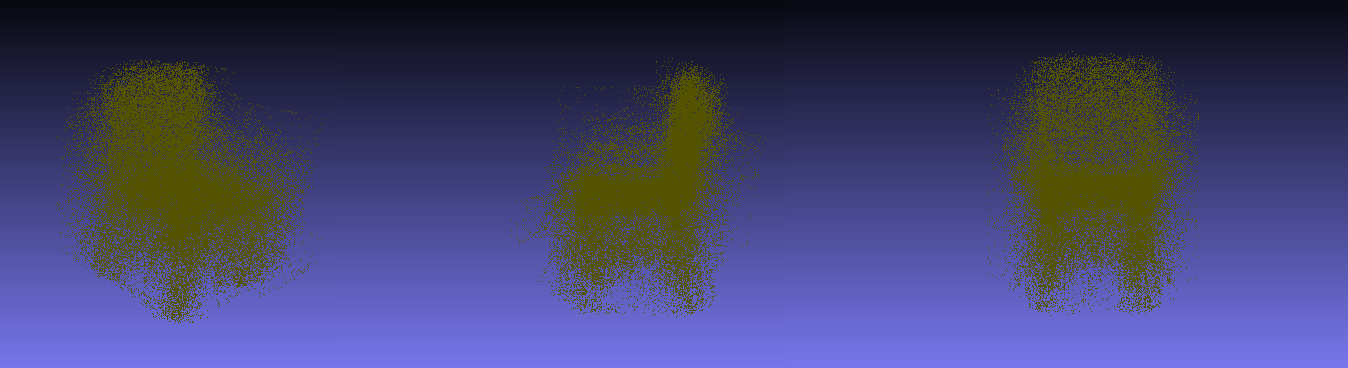
\includegraphics[width=0.8\textwidth]{chair_all.png}
	\caption{24 Stuhldaten in einen Koordinaten System geladen}
	\label{fig:Bild85}
\end{figure}
\newpage

\subsection{Ergebnisse - Versuchsaufbau 2}

Für Versuchsaufbau 2.1 vgl. \ref{sec:versuch2-aufbau} wurde zunächst der Autoencoder mit den zerstörten Blattdaten auf 500 Epochen trainiert. Um eine komprimierte Version auf 128-D zu erlernen. Dabei wurde zunächst die in Kapitel \ref{sec:autoencoder} vorgestellte Chamfer Distanz als Distanzmass genommen. Beispiel Trainingsdatensätze können  Abb. \ref{fig:Bild69} entnommen werden mit ihren den jeweiligen erzeugten Output des Decoders in Abb. \ref{fig:Bild68}. Wie zu erkennen ist vervollständigt der Autoencoder mit der Chamfer Zielfunktion die Blätter selbstständig obwohl das nicht als Ziel in diesen Bearbeitungsschritt ist. Es ist zu erkennen, dass die Dichte in welche die Punkte beim Output auf der Höhe der Löcher angeordnet ist stark von den üblichen Bereichen auf den Blatt abweicht. Auch lässt der Trainingsverlauf in Abb. \ref{fig:Bild67} darauf schließend das selbst beim weiteren Training der Autoencoder keine bessere Codierung erlernen wird, welche die Löcher in den Blättern erzeugt, da seit Epoche 300 das Training stagniert. Außerdem lassen das durch die Chamfer Distanz berechnete Abstand zwischen den beiden Punktwolken keine starke Verbesserung mehr zu da die durchschnittliche Diskrepanz nach dieser Metrik, zwischen den Input x und den von Decoder erzeugten Output x` nur noch im 0.0005 cm Bereich liegt nach wie in Abb.\ref{fig:Bild67} in Epoche 500 abzulesen ist. Da keine vernünftige Trainingsdaten für den Latenten C-GAN Versuchsaufbau 2.1 generiert werden können kann an dieser Stelle der Versuchsaufbau 2.1 Latent C-GAN  mit Chamfer Distanz nicht weiter geführt können. 

\begin{figure}[htbp] 
	\centering
	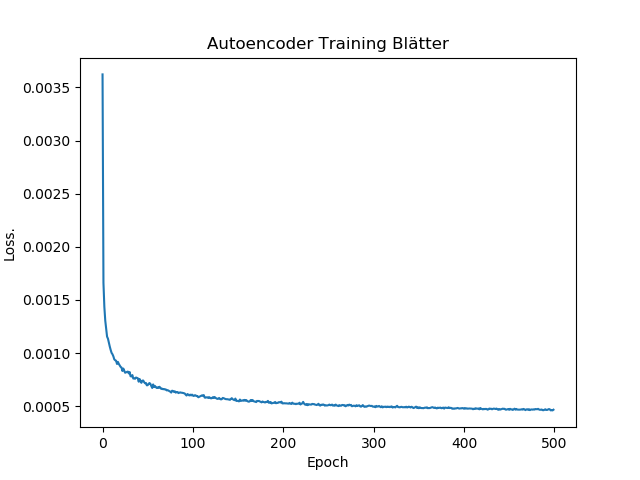
\includegraphics[width=0.6\textwidth]{autoencoder_training_blaetter_result.png}
	\caption{Trainingsverlauf des Autoencoder mit CD für zerstörte Blattdaten}
	\label{fig:Bild67}
\end{figure}

\begin{figure}[htbp] 
	\centering
	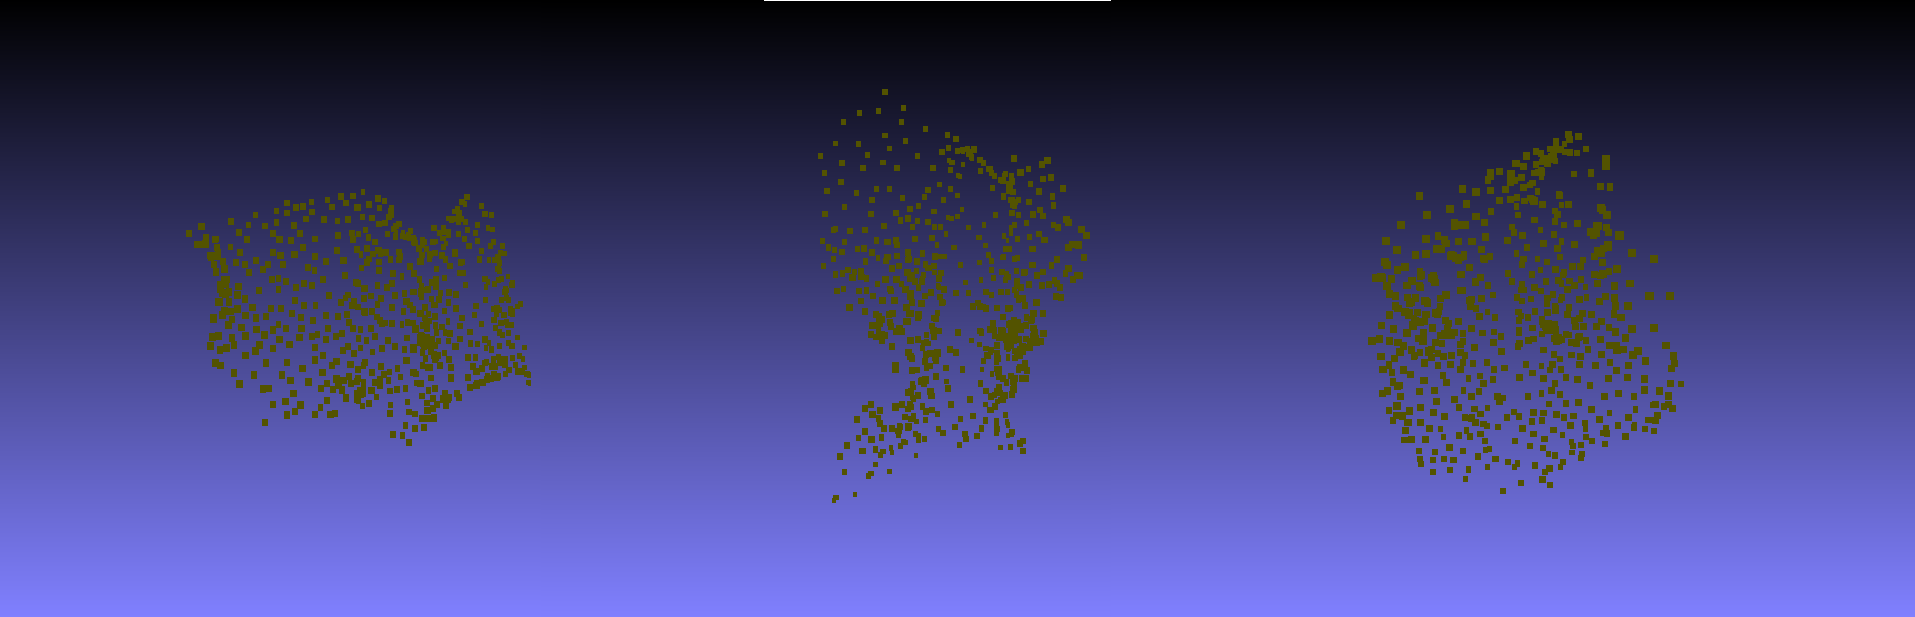
\includegraphics[width=1.0\textwidth]{autoencoder_destroyed_example_chamfer_fake.png}
	\caption{Trainingsbeispiele des Autoencoder mit CD für zerstörte Blattdaten - Output}
	\label{fig:Bild68}
\end{figure}

\begin{figure}[htbp] 
	\centering
	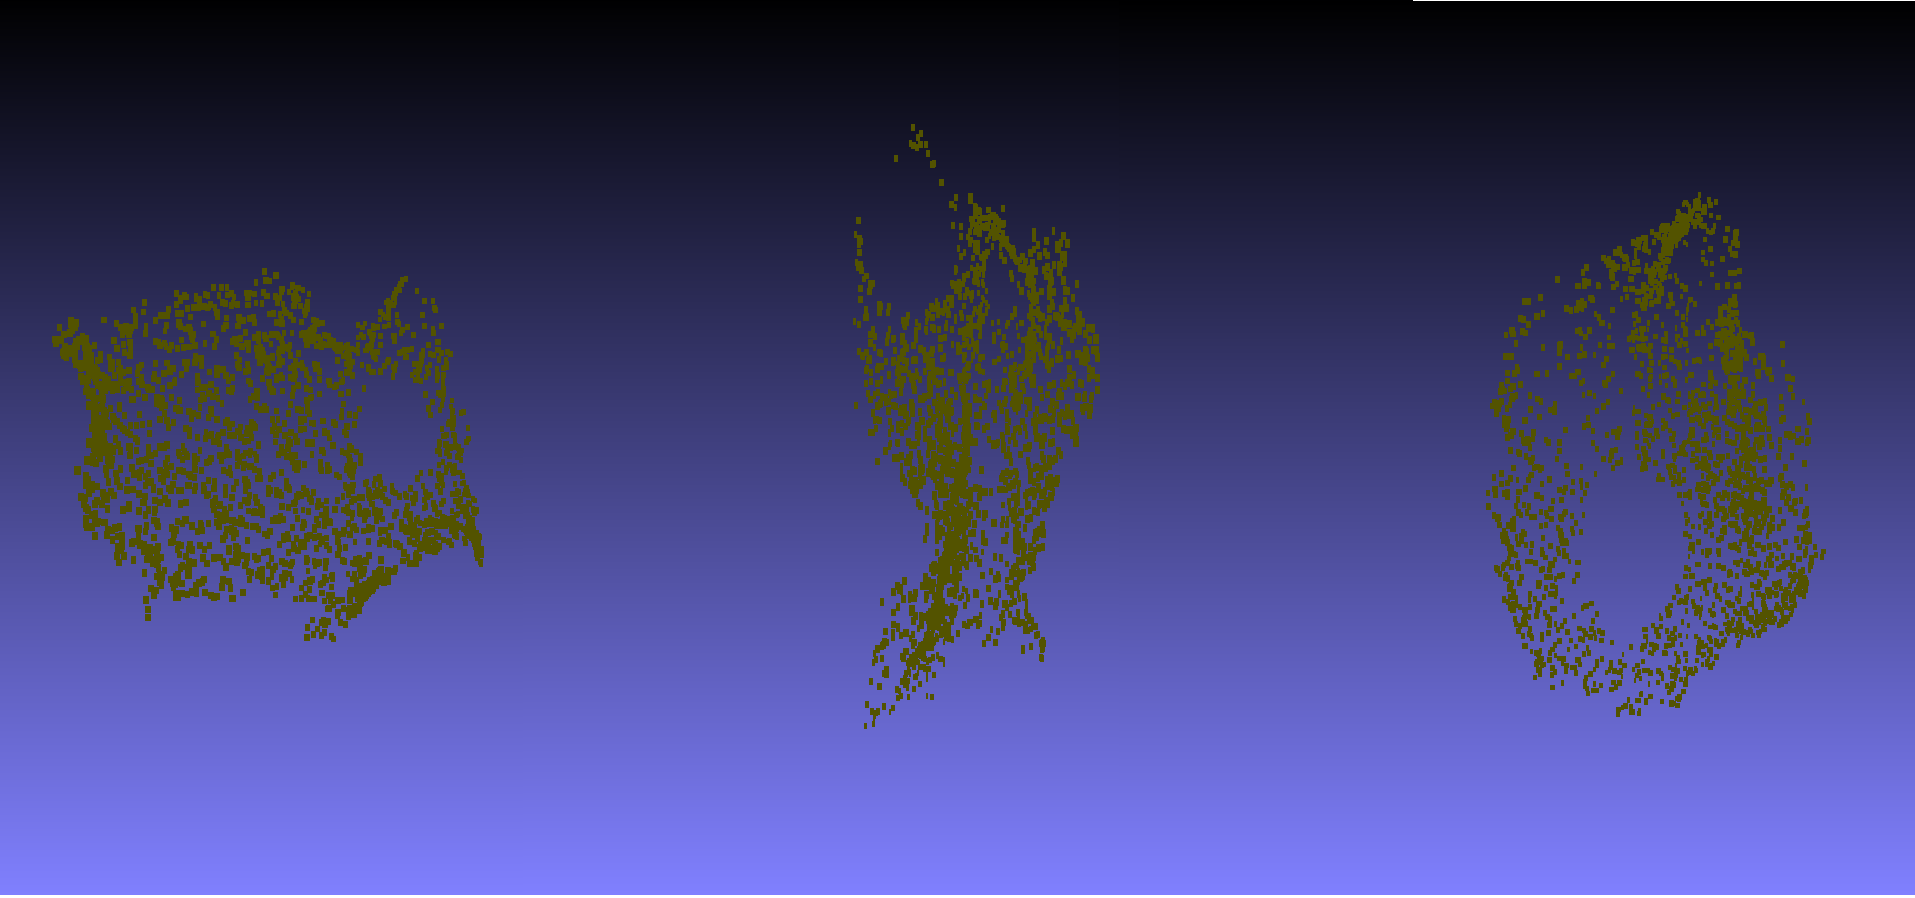
\includegraphics[width=1.0\textwidth]{autoencoder_destroyed_example_chamfer_real.png}
	\caption{Trainingsbeispiele des Autoencoder mit CD für zerstörte Blattdaten - Input}
	\label{fig:Bild69}
\end{figure}
\newpage

Um nun bessere Validierungsergebnisse zu erlangen wurde Versuchaufbau 2.1 latent-CGAN noch mit EMD Zielfunktion für Autoencoder getestet. Es wurden 800 Epochen trainiert. Die Ergebnisse sind recht ähnlich zu der mit der Chamfer Distanc vgl.\ref{sec:autoencoder}. Beispiel Trainingsinput Trainingsdatensätze können in Abb. \ref{fig:Bild71} entnommen werden mit den jeweiligen erzeugten Output des Decoders in Abb. \ref{fig:Bild72} entnommen. Wie zu erkennen ist, vervollständigt der Autoencoder mit der EMD die Blattflächen selbstständig obwohl das nicht als Ziel des Autoencoder ist, sondern nur das lernen einer Kodierung. Im Vergleich dazu sind die Blätter aber an der Stelle des Loches gleichmäßiger Verteilt und es gibt keine höheren Punktansammmlungen auf der Blattfläche. Wenn man die Ergebnisse mit der Hinsicht der Zielfunktion berücksichtigt liefert die CD ein besseres Ergebnis. Mit der Begründung das auf der Blattoberfläche die Blätter gleichmässiger Verteilt wurden sind. Möchte man nun die beiden Ergebnisse ebenfalls auf die Qualität des Rekonstruieren messen obwohl dies nicht das eigentliche Ziel ist sticht die EMD hervor da auch auf in den Bereich der Löcher die Punkte gleichmäßiger Verteilt sind.
\\\\
Insgesamt sind die Distanzen niedriger und die Dichte an den Löchern nimmt ab. Jedoch liefert die EMD bessere den besseren Nebeneffekt das die Blätter realistischer Rekonstruiert werden. \ref{fig:Bild67} darauf schließend das selbst beim weiteren Training nicht die Löcher welche in den Blättern sind herzustellen sind, da seit Epoche 300 das Training stagniert. Außerdem lassen das durch die Chamfer Distanz berechnete Abstand zwischen den beiden Punktwolken keine starke Verbesserung mehr zu da die durchschnittliche Diskrepanz zwischen den Input x und den von Decoder erzeugten Output x` nur noch im 0.03 cm Bereich liegt wie in Abb.\ref{fig:Bild67} in Epoche 500 abzulesen ist. Das Training entwickelt sich jedoch seit mehren Epochen nicht mehr und stagniert. Auch mit dieser Anwendung kann das latente C-GAN nicht weitergeführt werden da keine erfolgreichen Trainingsdaten erzeugt werden konnten.

\begin{figure}[htbp] 
	\centering
	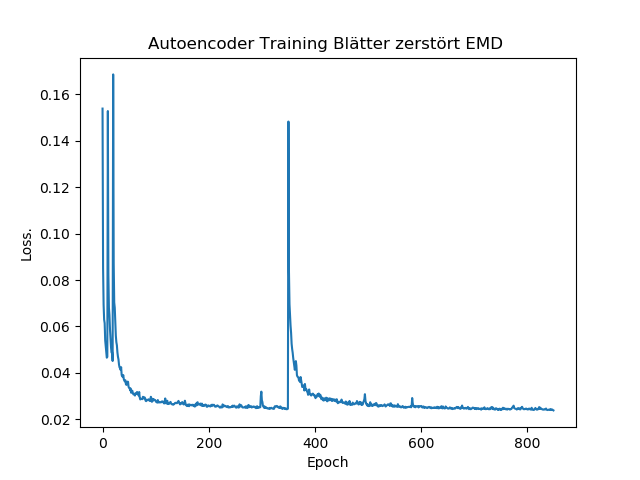
\includegraphics[width=1.0\textwidth]{autoencoder_training_bleatter_zer_result_emd.png}
	\caption{Trainingsverlauf des Autoencoder mit EMD für zerstörte Blattdaten }
	\label{fig:Bild71}
\end{figure}
\begin{figure}[htbp] 
	\centering
	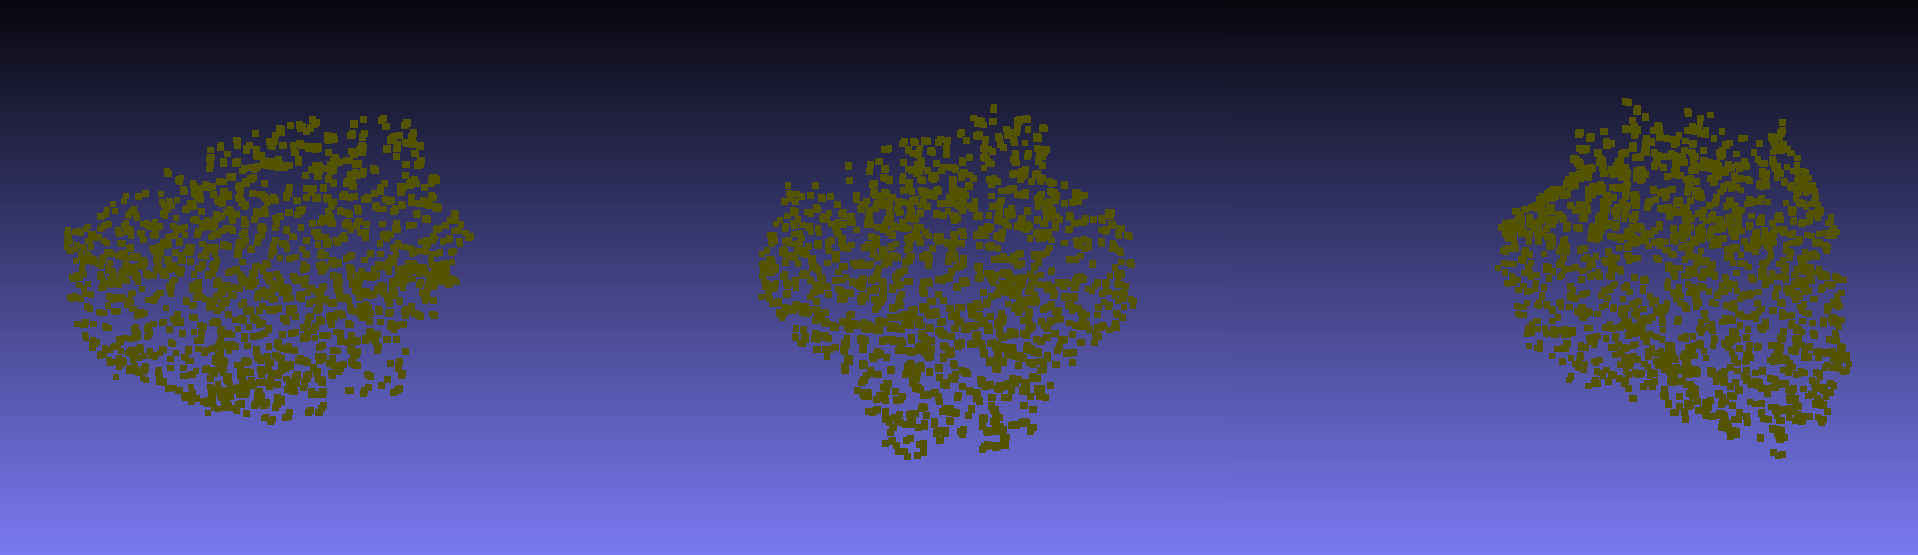
\includegraphics[width=1.0\textwidth]{repairded_emd.png}
	\caption{Trainingsbeispiele des Autoencoder mit EMD für zerstörte Blattdaten - Output}
	\label{fig:Bild72}
\end{figure}
\begin{figure}[htbp] 
	\centering
	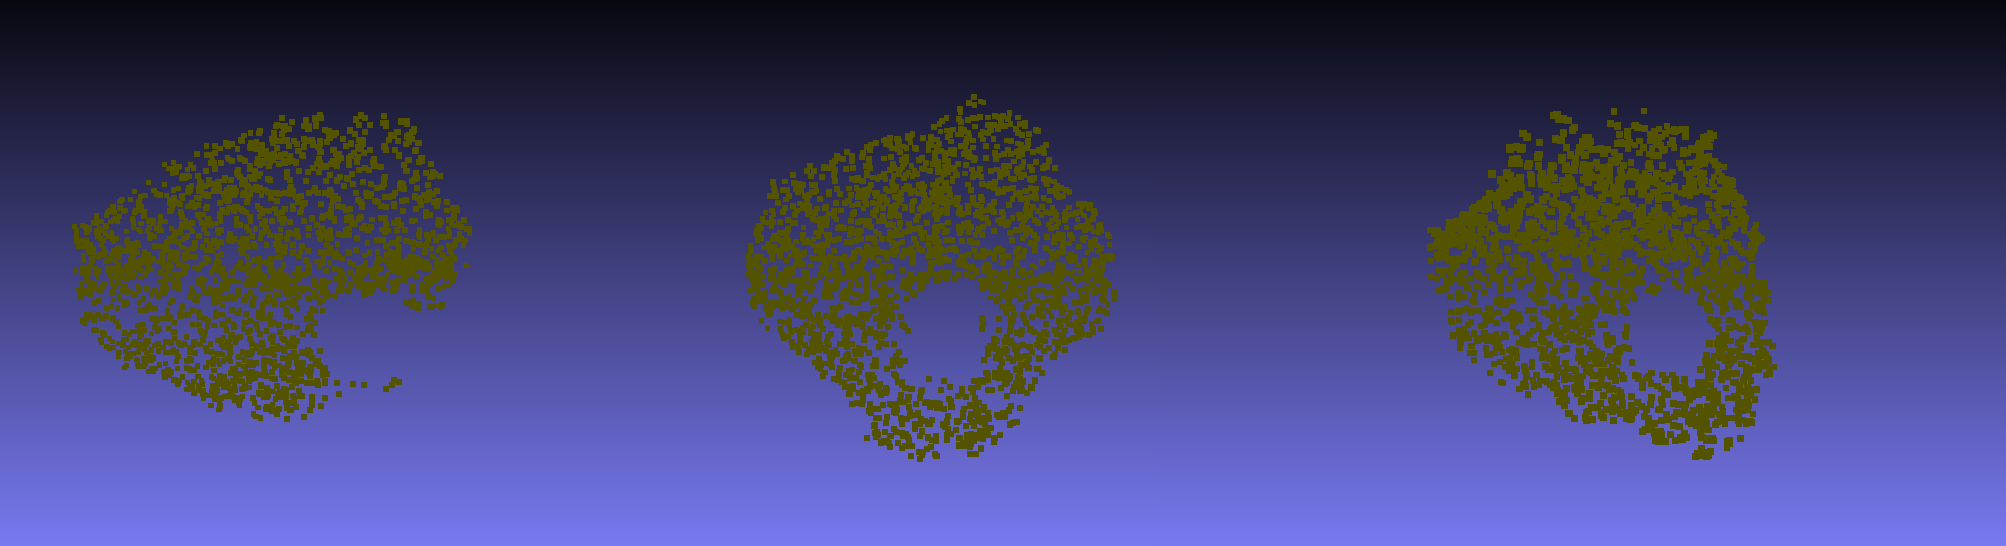
\includegraphics[width=1.0\textwidth]{input_emd.png}
	\caption{Trainingsbeispiele des Autoencoder mit EMD-Distanz für zerstörte Blattdaten - Input}
	\label{fig:Bild69}
\end{figure}
\newpage

Für den Versuchsaufbau 2.2 RAW-CGAN mit Fully-Connected-Layern mit Wasserstein Metric ist in Abb. \ref{fig:Bild75} ist rechts der Loss des Discriminators abgebildet und links der Loss des Generators. Der Loss des Generator sinkt zwar aber die generierten Trainingsbeispiele in Abb. \ref{fig:Bild77} ähneln keine reparierten Blätter.  Der dazugehörige Input ist in Abb.\ref{fig:Bild76} zu sehen. Da der Generator schon an sein Limit gerät und keine erhebliche Verbesserung mehr Möglich ist, ist festzustellen das durch einen Generator mit Fully-Connected-Layern keine Blattdatenrekonstruktion statt finden kann. 

\begin{figure}[htbp] 
	\centering
	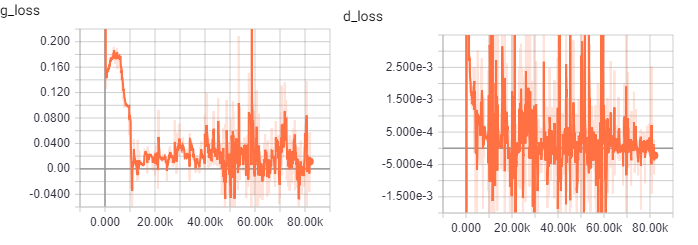
\includegraphics[width=1.0\textwidth]{wasserstein_fully_connected_rawcgan_loss.png}
	\caption{Generator und Discriminator Loss des RAW-CGAN mit Wasserstein Distanz}
	\label{fig:Bild75}
\end{figure}

\begin{figure}[htbp] 
	\centering
	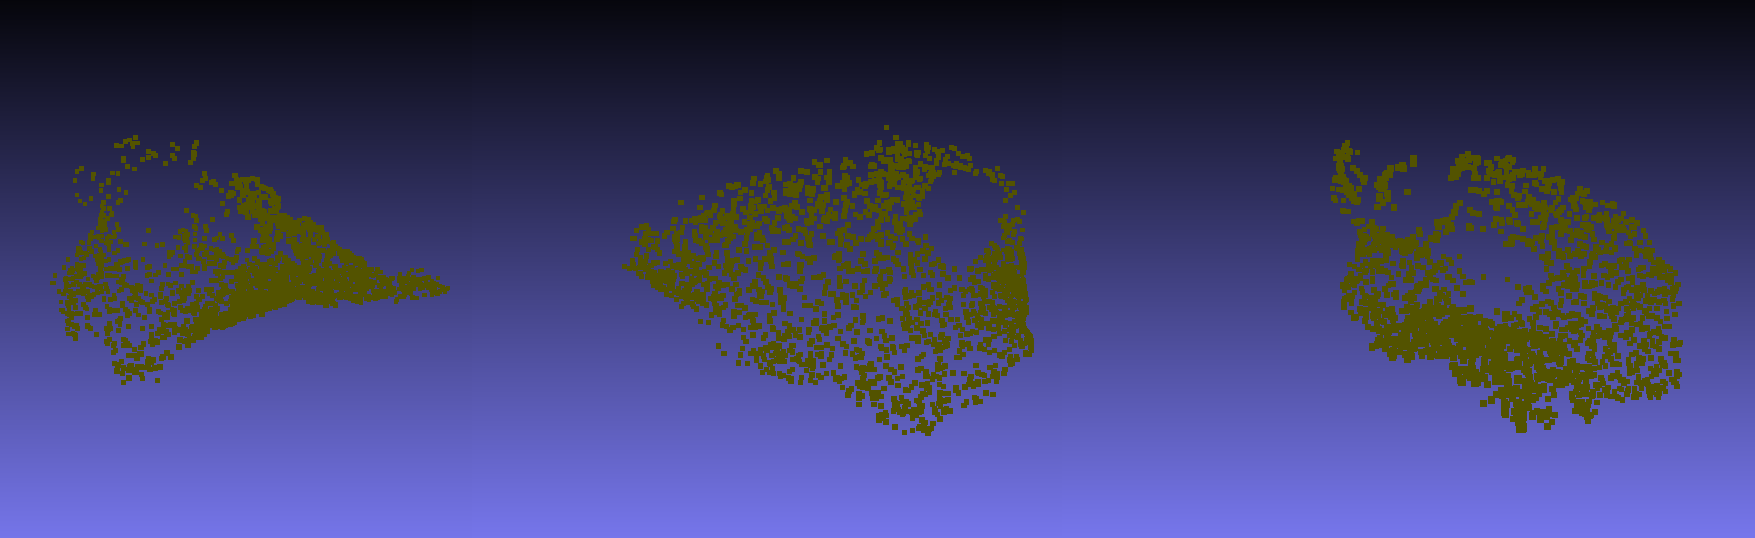
\includegraphics[width=0.5\textwidth]{reaf_fully_connected_wgan_.png}
	\caption{Der Input aus welchen vom RAW-CGAN die Daten rekonstruiert wurden}
	\label{fig:Bild76}
\end{figure}

\begin{figure}[htbp] 
	\centering
	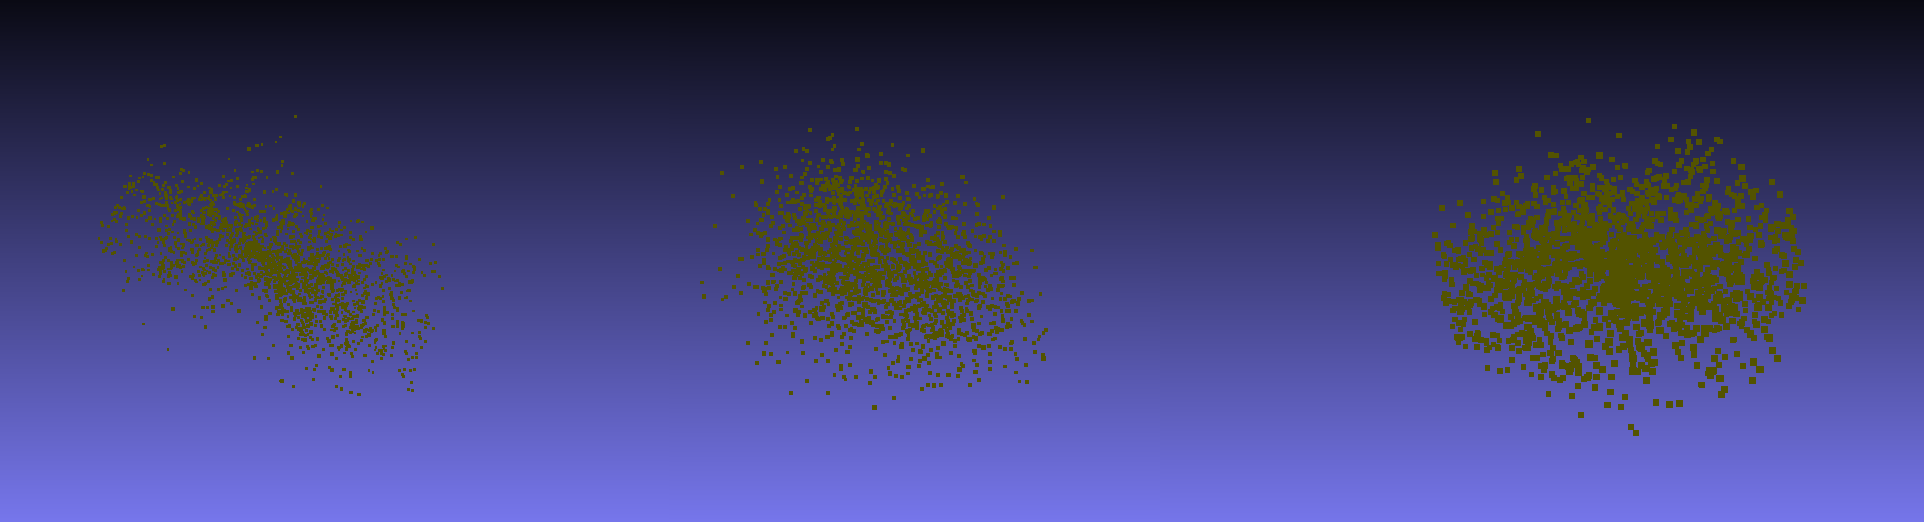
\includegraphics[width=0.5\textwidth]{fake_wgan_fully_rawcgan.png}
	\caption{Vom Generator des RAW-CGAN rekonstruierte Daten}
	\label{fig:Bild77}
\end{figure}
~\\\\
Als nächtest  erfolgen die Ergebnisse von Testaufbau 2.2 RAW-CGAN mit Convolutional Layer im Discriminator und der Vanilla-GAN-Loss. Der Trainingsverlauf vom Generator und Discriminator kann in Abb. \ref{fig:Bild79} entnommen werden. Die Sprünge schauen auf den ersten Blick sehr stark aus beachtet man aber die Scalenwerte auf der Y-Achse des Generators bewegt sich der Loss zwischen 0.691 und 0,696. Dies lässt auf keine starke Verbesserung schließen. Das Training läuft über mehre Epoche konstant hinweg und lässt auch für eine längeren Durchlauf auf keine Verbesserung schließen. Einige erstellten Beispieltabakblätter welche vom Generator erstellt wurden sind können aus Abb. \ref{fig:Bild80} zu entnehmen so wie der dazu gehörige Input aus Abb. \ref{fig:Bild78}. Diese sind jedoch keine hohe Ähnlichkeit zu Blätter zu erkennen. Und da es nach der Loss Funktion keine gravierenden Veränderungen mehr zu erwarten sind kann festgehalten werden das keine Rekonstruktion von zerstörten Blattdaten mit den in Kapitel \ref{sec:versuch2-aufbau} beschriebenen RAW-CGAN mit Convolutional-Layer und Vanilla-GAN-Loss möglich ist. 

\begin{figure}[htbp] 
	\centering
	\includegraphics[width=0.5\textwidth]{cgan_loss_vanilla.png}
	\caption{RAW-CGAN Loss}
	\label{fig:Bild79}
\end{figure}

\begin{figure}[htbp] 
	\centering
	\includegraphics[width=0.5\textwidth]{dcpgan_ws_fake.png}
	\caption{Der Output aus welchen vom RAW-CGAN mit Convolutional Layern die Daten rekonstruiert wurde}
	\label{fig:Bild80}
\end{figure}

\begin{figure}[htbp] 
	\centering
	\includegraphics[width=0.5\textwidth]{dc_pgan_ws_real.png}
	\caption{Der Input aus welchen vom RAW-CGAN mit Convolutional Layern die Daten rekonstruiert wurden}
	\label{fig:Bild78}
\end{figure}

Zuletzt erfolgen die Ergebnisse von Testaufbau 1.2 RAW-CGAN mit Deconvolutional-Layer mit der Wasserstein-Metric, welches mit den nicht komprimierten Daten trainiert wird. Dass heißt wie in \ref{sec:versuch2_daten} beschrieben Blattdaten. Der Trainingsverlauf vom Generator und Discriminator kann in Abb. \ref{fig:Bild81} entnommen werden. Aus den Verlauf des Discriminator Loss arbeitet sich konstant nach unten hat zwei Ausbrecher welche aber kein Einfluss auf den weiteren Trainingsverlauf hat. Der Generator springt zwar noch am Ende des Trainings aber die Sprünge sind in einen so niedrigen Intervall das keine große Veränderung mehr erwartet werden kann. Die vom Generator generierten Outputs in Abb. \ref{fig:Bild82} und deren dazugehöriger Input in Abb. \ref{fig:Bild83} zeigen schon die Umrisse der Blätter auf jedoch sind die Blattflächen nicht gebildet. 

\begin{figure}[htbp] 
	\centering
	\includegraphics[width=0.5\textwidth]{cgan_ws_loss.png}
	\caption{Discriminator und Generator Loss RAW-DGAN mit Convolutional-Layer und Wasserstein Distanz}
	\label{fig:Bild81}
\end{figure}

\begin{figure}[htbp] 
	\centering
	\includegraphics[width=0.5\textwidth]{raw_cgan_ws_fake.png}
	\caption{Der Output aus welchen vom RAW-CGAN mit Convolutional Layern die Daten rekonstruiert wurde}
	\label{fig:Bild82}
\end{figure}

\begin{figure}[htbp] 
	\centering
	\includegraphics[width=0.5\textwidth]{raw_cgan_ws_real.png}
	\caption{Der Input aus welchen vom RAW-CGAN mit Convolutional Layern die Daten rekonstruiert wurden}
	\label{fig:Bild83}
\end{figure}


Fast man nun Versuchsaufbau 2 zusammen. Ist festzustellen das in Versuchsaufbau 2.1 abgebrochen werden musste da die Autoencoder nicht fähig waren die zerstörten Trainingsdaten zu erlernen. Jedoch schafften sie die Daten zu rekonstruieren obwohl dies nicht als Ziel für die Autoencoder definiert wurde. Ob eine praktische Anwendung dadurch ermöglicht ist und ob diese Rekonstruktion nur für die Form für Blätter gilt oder auch Beispielsweise ähnliche Ergebnisse beim Stuhldaten Satz liefert muss geprüft werden. Die beiden Zielfunktionen des Autoencoder, CD und EMD, hatten beide ein ähnliches Problem welcher Punkt in Punktwolke x ist die dazugehörige Punkt in Punktwolke y. Beide lösten dies indem sie die nähsten Nachbarn eines Punktes suchen aus der anderen Punktwolke.  Jedoch für dieses Mapping zu Problemen führen wie man in Abb. erkennen kann. Die rote Punktwolke ist der erste Versuch des Autoencoder die grüne Punktwolke zu kopieren. Eine Zuordnung in diesem Stadium welcher Punkt in rot zu grün gehört ist sehr schwierig. Dadurch resultiert das Punkte in Zentrum eher als nächster Nachbar identifiziert werden. Und lassen in weiteren Trainingsverlauf die Punktwolke wie einen Teig außernander gehen und lassen es nicht zu die Löcher zu entstehen. Für eine weitere Nutzung könnte an dieser Stelle angestetzt werden und andere Zielfunktionen für Autoencoder mit Punktwolken entwickelt werden. 
\\\\
Im Versuchsaufbau 2.2 zeigen sich bessere Ergebnisse mit der Verwendung von Convolutional-Layer im Discriminator. Ein qualitativer Unterschied zwischen den Versuchsaufbau 2.2 RAW-CGAN mit Convolutional-Layer und Vanilla-GAN oder Wasserstein Metrik lässt sich nicht feststellen. Jedoch lässt durch die Convolutional-Layer das erlernen der Latenten-Struktur besser gelingen. Eine Rekonstruktion ist aber auch mit diesen Model nicht möglich. Jedoch kann nicht ausgeschlossen sein das GAN durch andere Aufbauten wie Beispielsweise mit 1D-Deconvolutional-Layer implementiert werden. Welche bei Tensorflow 1.12 als Prototyp zur Verfügung steht. Eine andere Möglichkeit wäre auf die Arbeit von Cai, Zhongang  und Yu \cite{3d-conv} anzusetzen dieser postuliert eine Methode für 3D-Convolution Methode welche auf 3D-Punktwolken arbeitet und eine Invarianz im Euklidischen Raum lernt mit deren Hilfe es leicht sein soll Rotationen der Punktwolke zu erlernen. Durch diese neuen Module könnte das erlernen des latenten Raumes von 3d-Punktwolken möglich gemacht werden und das letztendliche Ziel, 3D-Punktwolken zu rekonstruieren möglich gemacht werden. 
\newpage

\section{Zusammenfassung und Diskussion }

3D-Daten bleiben eine Herausforderung zu den vergleichsweise anderen Daten wie Bilder oder Audio da ihr Suchraum erheblich höher ist, dieses Thema wurde auch schon in Kapitel \ref{sec:3dprobleme} thematisiert. Die beiden Ziele:
 
\begin{description}
	\item[Ziel 1]
	Können durch GANs 3D-Punktwolken von Tabakblättern erlernt werden um neue Datensätze zu generieren?\\
	\item[Ziel2]
	Können durch GANs 3D-Punktwolken von Tabakblättern welche von Tabakblättern von ihren Urzustand abgebracht wurden rekonstruiert werden? 
\end{description}


welche in dieser Arbeit überprüft wurden, ist festzuhalten das Ziel 1 durch GANs machbar ist jedoch noch Verbesserungen in der Qualität möglich sind. Diese können durch Beispielsweiße, erhöhung der Trainingsdaten, eine Datenvorverarbeitung welche den Suchraum einschränkt oder Verbesserung des GAN Modells durch verwendung von 1D- deconvolutional-Layer oder 3D-Convolutional-Layer für Punktwolken \cite{3d-conv} möglicher weiße erreicht werden. 
\\\\
Für Ziel 2 welches in Kapitel \ref{sec:versuch2-aufbau} überprüft wurde ist festzuhalten das der Aufbau des Latent-CGAN abgebrochen werden musste, da der Autoencoder es nicht geschafft das die zerstörten Trainingsdaten zu erlernen. 


auch zeigt beispielsweiße bei der Rekonstruction von Bildern das erst durch den Einsatz verbesserter Convolution Methoden es erst Möglich gemacht wurde Bilder zu rekonstruieren und zu verändert \cite{imagerecon}.

Eine weitere Möglichkeit ist das Konzept welches Zhu, Jun-Yan und Park \cite{pix2pix}, mit ihren Pix2Pix Model vorgestellt haben. In dieser Verwendet sich die C-GAN Loss Funktion und ändern diese um Zusätzlich zu der üblichen Loss-Funktion die Differenz zwischen Generator Output und den dazugehörigen Urzustand Trainingsdatensatz zu berechnen und addieren dies zu der Loss-Funktion. Der Optimizer versucht nun dieses Differenz zusätzlich zu Minimieren. Man könnte dieses Verfahren nun für Punktwolken übernehmen und mit der CD oder EMD implementieren. 


Fast man nun Versuchsaufbau 2 zusammen. Ist festzustellen das in Versuchsaufbau 2.1 abgebrochen werden musste da die Autoencoder nicht fähig waren die zerstörten Trainingsdaten zu erlernen. Jedoch schafften sie die Daten zu rekonstruieren obwohl dies nicht als Ziel für die Autoencoder definiert wurde. Ob eine praktische Anwendung dadurch ermöglicht ist und ob diese Rekonstruktion nur für die Form für Blätter gilt oder auch Beispielsweise ähnliche Ergebnisse beim Stuhldaten Satz liefert muss geprüft werden. Die beiden Zielfunktionen des Autoencoder, CD und EMD, hatten beide ein ähnliches Problem welcher Punkt in Punktwolke x ist die dazugehörige Punkt in Punktwolke y. Beide lösten dies indem sie die nähsten Nachbarn eines Punktes suchen aus der anderen Punktwolke.  Jedoch für dieses Mapping zu Problemen führen wie man in Abb. erkennen kann. Die rote Punktwolke ist der erste Versuch des Autoencoder die grüne Punktwolke zu kopieren. Eine Zuordnung in diesem Stadium welcher Punkt in rot zu grün gehört ist sehr schwierig. Dadurch resultiert das Punkte in Zentrum eher als nächster Nachbar identifiziert werden. Und lassen in weiteren Trainingsverlauf die Punktwolke wie einen Teig außernander gehen und lassen es nicht zu die Löcher zu entstehen. Für eine weitere Nutzung könnte an dieser Stelle angestetzt werden und andere Zielfunktionen für Autoencoder mit Punktwolken entwickelt werden. 
\\\\
Im Versuchsaufbau 2.2 zeigen sich bessere Ergebnisse mit der Verwendung von Convolutional-Layer im Discriminator. Ein qualitativer Unterschied zwischen den Versuchsaufbau 2.2 RAW-CGAN mit Convolutional-Layer und Vanilla-GAN oder Wasserstein Metrik lässt sich nicht feststellen. Jedoch lässt durch die Convolutional-Layer das erlernen der Latenten-Struktur besser gelingen. Eine Rekonstruktion ist aber auch mit diesen Model nicht möglich. Jedoch kann nicht ausgeschlossen sein das GAN durch andere Aufbauten wie Beispielsweise mit 1D-Deconvolutional-Layer implementiert werden. Welche bei Tensorflow 1.12 als Prototyp zur Verfügung steht. Eine andere Möglichkeit wäre auf die Arbeit von Cai, Zhongang  und Yu \cite{3d-conv} anzusetzen dieser postuliert eine Methode für 3D-Convolution Methode welche auf 3D-Punktwolken arbeitet und eine Invarianz im Euklidischen Raum lernt mit deren Hilfe es leicht sein soll Rotationen der Punktwolke zu erlernen. Durch diese neuen Module könnte das erlernen des latenten Raumes von 3d-Punktwolken möglich gemacht werden und das letztendliche Ziel, 3D-Punktwolken zu rekonstruieren möglich gemacht werden. 

\newpage
\listoffigures
\newpage
\bibliographystyle{apacite}
\bibliography{mybib}
\end{document}
